\documentclass[a4paper,10pt,abstracton,notitlepage]{scrreprt}
\usepackage[utf8]{inputenc}
\usepackage{fullpage}
\usepackage{hyperref}
\usepackage{isomath}
\usepackage{amsfonts}
\usepackage{amsmath}
\usepackage{graphicx}
\usepackage{float}
\usepackage{wrapfig}
\usepackage{caption}
\usepackage[export]{adjustbox}
\usepackage{gnuplottex}
\usepackage[mathcal]{euscript}
\usepackage{siunitx}
\usepackage{algpseudocode}


\captionsetup{font={small}}

\title{Dynamic loading of 3D models}
\subtitle{PROJ-H-402 Project Report}
\author{Tim Lenertz, INFO MA1, ULB}
\date{\today}

\begin{document}

\maketitle{}

\vspace{3cm}
\renewcommand{\abstractname}{Résumé}
\begin{abstract}
Des fichiers nuage de points produits par des scanneurs 3D actuels peuvent aisément devenir trop lourds pour pouvoir être traités ou visualisés en entier. Ce projet met en comparaison plusieurs structures de données, formats de fichier et techniques de filtrage qui pourraient permettre d'en extraire dynamiquement des sous-ensembles rélévants. Sur cette base une application a été développée qui créé une telle structure et permet à l'utilisateur de se déplacer à travers et d'explorer un nuage de points de grande taille.
\end{abstract}

\vspace{2cm}
\renewcommand{\abstractname}{Abstract}
\begin{abstract}
Point cloud data produced by current 3D scanning technology can quickly become too large in size to be processed or visualized as a whole. This project compares several data structures, file formats and filtering techniques that would make it possible to dynamically extract relevant subsets. Based on this an application was developped which creates such a structure and allows the user to seamlessly move through and explore areas of a large point cloud. 
\end{abstract}

\tableofcontents{}

\chapter{Introduction}
Point clouds are a way of digitally representing three-dimensional models using only a set of points located on the object's surfaces\footnote{Only non-volumetric point clouds are considered for this project. In volumetric point clouds, points are not only located on surfaces, but on the insides of objects.}. Each point consists of 3 coordinates $(x, y, z)$ on an Euclidian coordinate system defined for the model, and can be attributed with additional information such as color, surface normal vector, and others.

This data is typically produced by 3D scanners, which today can capture surfaces at a very high level of detail and thus yield huge quantities of points. Full representations of large objects or environments can be synthesized by combining the outputs of multiple scans from different view points. For example to get a full point cloud model of an archeological site, aerial scans may be combined with close-up scans of individual landmarks. The resulting files can easily reach several GB in size and contain over $10^{8}$ points, and so they can no longer be processed or visualized efficiently as a whole. Instead, subsets of points around an area of interest are extracted.

The goal of this project is to develop a system which dynamically loads the visible subset of points to render, while the user moves through a large point cloud. This involves filtering methods to extract the right subsets from the point cloud, the data structure which the full point cloud is stored in, and the file format using which this data structure is serialized on the storage device. The process should appear seamless to the user.

To this end, different data structures and file formats were compared for their possibilities to extract the right subsets of points in an efficient way, and a program was developped which converts a given point cloud file into such a data structure, and then allows the user to explore the point cloud, by dynamically loading chunks of it from the preprocessed data structure file.

\begin{figure}[H]
\centering
	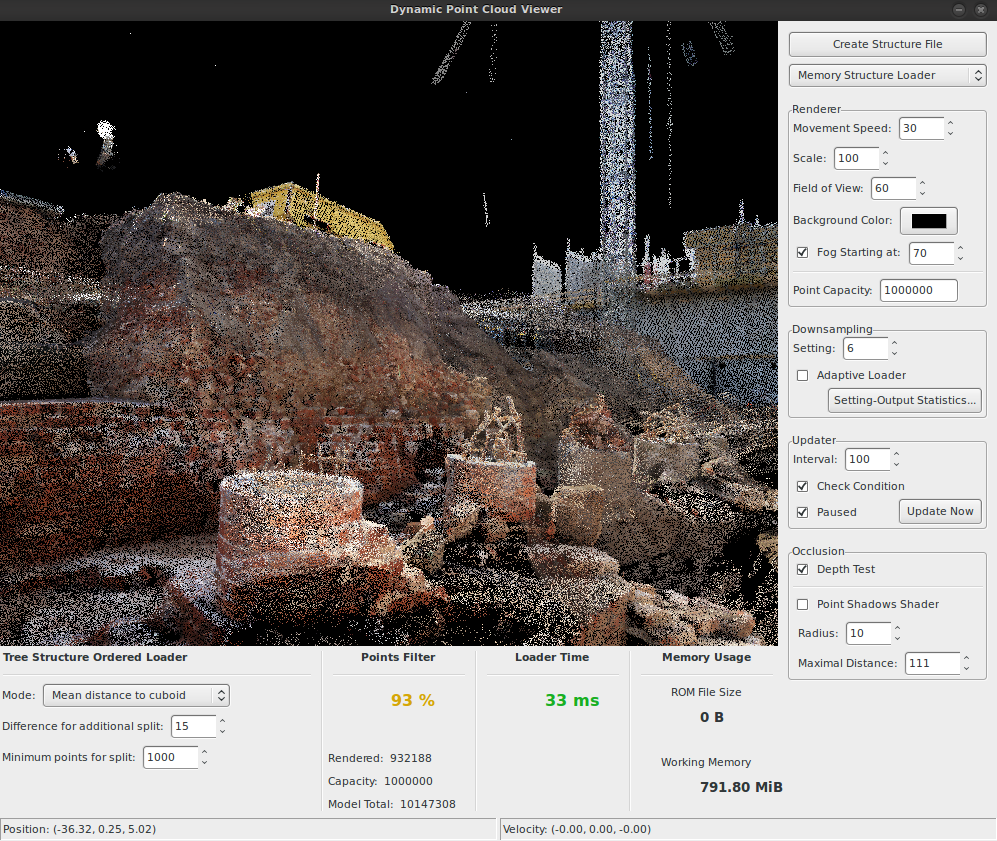
\includegraphics[height=9cm]{screenshot.png}
	\caption{Screenshot of the \emph{Viewer} application}
\end{figure}



\chapter{Filtering the point cloud}
This chapter describes the methods used to compute a smaller set of points based on the full point cloud, that should still visually reproduce the model as seen from a given view point. The data structure used to store the point cloud is not considered in this chapter.

\section{Definitions}
The following definitions are used throughout this report. A \emph{point cloud} is an unordered set of points with an Euclidian coordinate system. Each \emph{point} $p = \langle x, y, z, r, g, b\rangle$ consists of its coordinates $x, y, z$, and RGB color information. The \emph{model} $P$ is the full point cloud used as input. The \emph{point capacity} $C$ is the maximal number of points that can be outputted to the renderer. 

The \emph{view-projection matrix} $\matrixsym{M} = \matrixsym{P} \times \matrixsym{V}$ is a 4x4 matrix that defines the view frustum of the camera. The 6 planes of the frustum can be derived from the matrix as described in \ref{sec:frustum_planes}. The \emph{view matrix} $\matrixsym{V}$ transforms the points' coordinate system into one centered around the camera at its current position and orientation, while the \emph{projection matrix} $\matrixsym{P}$ is used to project the points to their two-dimensional screen coordinates. $\matrixsym{P}$ might define both a parallel projection or a perspective projection with a given \emph{field of view} $\lambda$.

The \emph{filtering function} $f_{P}(\matrixsym{M})$ computes a set of rendered points $P'$ from the model $P$, the matrix $\matrixsym{M}$, and additional parameters. Its main constraint is that $|P'| \leq C$ (whereas $|P|$ may be much larger than $C$). $P'$ does not need to be a subset of $P$: Some methods (such as uniform downsampling) will add points into $P'$ that are not in $P$, in order to achieve a better visual quality.

The criteria for quality of the filtering function is that the 2D projection of $P'$ at the current view point $\matrixsym{M}$ looks similar to that of $P$, that is there should be no loss of important details and no obvious visual artifacts or discontinuities. Techniques such as hidden surface removal could actually improve the appearance of $P'$ compared to that of $P$.

The function $f_{P}$ described in this chapter is an idealized version that operates on a set of points. The next chapters describe algorithms that implement $f_{P}(\matrixsym{M})$ using a specific data structure for $P$, and with additional time complexity constraints.


\section{Projection}
When the point cloud is rendered, the points $p$ are projected from their three-dimensional virtual space onto the two-dimensional screen, using the view frustum defined by $\matrixsym{M}$. This can be described as a function $\mathrm{proj}_{\matrixsym{M}}(x, y, z) = (x_{\mathrm{screen}}, y_{\mathrm{screen}})$, where $x_{\mathrm{screen}} \in [0, w[$ and $y_{\mathrm{screen}} \in [0, h[$, with $w$ and $h$ being the width and height of the screen in pixels. This operation is done on the GPU to render vertices.

First a vector in homogeneous coordinates is build from $x, y, z$: $\overrightarrow{p} = [x, y, z, 1]^{T}$. The fourth component $w = 1$ indicates that this vector represents a point in space; with $w = 0$ it would indicate a direction. In general, a point in homogeneous coordinates $[x, y, z, w]$ corresponds to $[\frac{x}{w}, \frac{y}{w}, \frac{z}{w}]$ in Euclidian coordinates. This allows for building transformation matrices that distinguish between points and vectors (notably for translations), and the projection matrix $\matrixsym{P}$.

Next $\overrightarrow{p}$ is multiplied by $\matrixsym{M}$: $\overrightarrow{p'} = \matrixsym{M} \times \overrightarrow{p} = \matrixsym{P} \times \matrixsym{V} \times \overrightarrow{p}$. The view matrix $\matrixsym{V}$ represents the position and orientation of the camera in the virtual space, so the first multiplication puts $\overrightarrow{p}$ into a coordinate system centered around the camera. The $w$ component remains $1$. It is then multiplied by $\matrixsym{P}$, which can change $w$. Finally the resulting $\overrightarrow{p'}$ is transformed back into Euclidian coordinates to yield the camera coordinates $x_{\mathrm{cam}}, y_{\mathrm{cam}}, z_{\mathrm{cam}}$. In the case of perspective projection, foreshortening is done with the component-wise division by $w$. Because this is a non-affine transformation, it could not be done using 3x3 matrix arithmetic alone.

Camera coordinates are considered to be inside the view frustum only if $x_{\mathrm{cam}}, y_{\mathrm{cam}}, z_{\mathrm{cam}} \in [-1, 1]$, and then the two-dimensional screen coordinates $x_{\mathrm{screen}}, y_{\mathrm{screen}}$ are deduced by linearly mapping $x_{\mathrm{cam}}$ and $y_{\mathrm{cam}}$ to $[0, w[$ and $[0, h[$, respectively. $z_{\mathrm{cam}}$ no longer affects the position of the pixel, but comparing two values for $z_{\mathrm{cam}}$ indicates whether one point is in front of or behind another one in camera space, and is for example used in OpenGL's depth testing.

If $\matrixsym{P}$ is the identity matrix, it represents an orthographic projection where the view frustum is the axis-aligned cube from $[-1, -1, -1]$ to $[1, 1, 1]$. An orthogonal projection with a different cuboid frustum can be expressed by letting $\matrixsym{P}$ be a transformation matrix that maps coordinates in that cuboid to the former cube. The perspective projection matrix for field of view $\lambda$, screen aspect ratio $w/h$, and near and far clipping planes $z_{\mathrm{near}}$ and $z_{\mathrm{far}}$ is defined by:

\begin{displaymath}
\matrixsym{P} = \begin{bmatrix}
\frac{f}{w/h} & 0 & 0 & 0 \\
0 & f & 0 & 0 \\
0 & 0 & \frac{z_{\mathrm{far}} + z_{\mathrm{near}}}{z_{\mathrm{near}} - z_{\mathrm{far}}} & \frac{2 \times z_{\mathrm{far}} \times z_{\mathrm{near}}}{z_{\mathrm{near}} - z_{\mathrm{far}}} \\
0 & 0 & -1 & 0
\end{bmatrix}
\text{ with }
f = \frac{1}{\tan(\frac{\lambda}{2})}
\end{displaymath}


\section{Frustum culling}
The simplest and most effective filtering done by $f_{P}$ is \emph{view frustum culling}, which removes all points from $P$ that are not within the view frustum defined by $\matrixsym{M}$. This usually eliminates more than half of the points from the model: Those behind the viewer, those outside his field of view, and those too far away (beyond the far clipping plane $z_{\mathrm{far}}$). It is done implicitly by the GPU, but the goal of the filtering is to reduce the number of points before they are sent to the GPU.

Frustum culling can be done per point by clipping the camera coordinates as described above, but depending on the data structure used, entire regions of the model space will be tested to be inside or outside the frustum instead.


\section{Downsampling} \label{sec:downsampling}
Downsampling reduces the density of points. Because of foreshortening in perspective projection, sections of the model that are farther away from the camera will become smaller in the two-dimensional projection, and as a consequence their number and density of points increases. Since a smaller density is sufficient to visually represent the model, it makes sense to apply downsampling on regions of the point cloud, depending on their distance from the camera.

Because the point cloud is non-volumetric, points are distributed on two-dimensional surfaces of the three-dimensional model. So the density can be defined as the number of points per surface area $\rho = n/A$. This value remains unknown, because the program does not know or try to find the shapes of the surfaces. Because of the way the point clouds are generated, $\rho$ will remain approximately constant on small scale, but on composite point clouds that combine different scans, $\rho$ can vary greatly in different regions of the point cloud. Some objects could have been scanned close-up, while the surrounding environment has a much lower resolution. 

The level of downsampling is determined by a function $r(d)$ which gives a ratio in function of a distance to the camera. A downsampling algorithm will transform the point cloud such that at any position $\overrightarrow{p}$ (assumed to be located on a surface), the new density becomes $\rho' = r(d(\overrightarrow{p})) \times \rho$ (with $r \in [0, 1]$).

\subsection{Weighted points}
One method of doing downsampling is to assign a weight $w \in [0, 1]$ to each point $p \in P$, and let the downsampled set of points be the subset $P' = \{ p \in P : w(p) < r(d(p)) \}$. For this to work the weights $w$ need to be uniformly distributed among the points.

This leads to a continuous $\rho'$, so no visual discontinuities are produced. Also, if the data structure contains the weighted points $P$ in a list ordered by ascending $w$, then it is possible to dynamically extract $P'$ in time $O(|P'|)$.

\begin{wrapfigure}{r}{7cm}
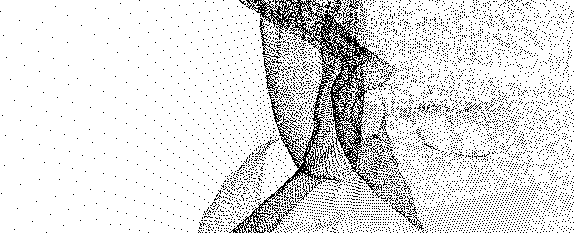
\includegraphics[width=7cm,frame]{random_weights_inv.png}
\caption{Weighted points downsampling using random weights}
\label{fig:random_weights}
\end{wrapfigure}
A simple way to distribute the weights is to set each weight to a random value. However, this leads to an irregular visual pattern in the way downsampled points are placed on the surfaces, as seen in figure \ref{fig:random_weights}. The left-hand side of the point cloud is not downsampled and retains the original regular pattern from the model.

\subsection{LOD regions}
Another possibility is to first compute several downsampled point sets $P'_{r}$ with fixed downsampling ratios $r$, during preprocessing. $P'$ is then produced out of pieces of these sets. The resulting $P'$ is thus composed of several \emph{level of detail} (LOD) regions\footnote{These are called \emph{mipmaps} in the implementation}, and so $\rho'(d)$ becomes a non-continuous staircase function, and visual discontinuities are produced. However, this method allows for producing the sets $P'_{r}$ without time constraints, and with a constant $r$.

In figure \ref{fig:uniform_example}, the region farther away was downsampled this way (using uniform downsampling). A visual discontinuity can be seen in the lower-right corner.

\subsection{Uniform downsampling}
Uniform downsampling is a downsampling algorithm that aims to produce a more regular pattern in the distribution of points on $P'$, as opposed to that produced by random downsampling (figure \ref{fig:random_weights}). It operates using a constant ratio $r$.

\begin{wrapfigure}{r}{7cm}
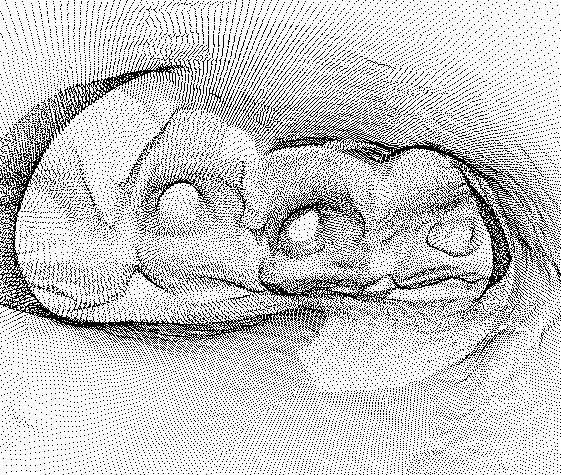
\includegraphics[width=7cm,frame]{uniform_example_inv.png}
\caption{Example of uniform downsampling}
\label{fig:uniform_example}
\end{wrapfigure}
The input point set $P$ is divided into a regular grid of cubes $C_{i,j,k}$ with side length $l$. For all cubes that contain at least one point, exactly one single point $p'$ is outputted into $P'$, whose position is the mean of that of the points in $C$, and whose color is that of the point $p \in P$ closest to that position. Figure \ref{fig:uniform_algo} illustrates the procedure in two dimensions. The more regular aspect of $P'$ is because its points are constrained by the regular grid. The algorithm also does not require $P$ to have a regular pattern to begin with.

The main difficulty is to find the value for the side length $l$, such that $n = |P'|$ is approximately equal to $r \times |P|$. Figure \ref{fig:uniform_stat} shows how $n$ varies in function of $l$ for some example models: In general, $n$ gets larger as the side length $l$ gets smaller, because there are more cubes available in the region of the model. Because the cubes are non-overlapping and each point $p \in P$ belongs to exactly one cube, $n$ is at most $|P|$. It reaches this value once $l$ reaches a value (depending on the density) where each point belongs to a different cube.

However, the function is not entirely monotonic, as the close-up view in figure \ref{fig:uniform_stat_detail} shows. This is because when $l$ gets changes, all cubes on the grid (except those at the origin) get displaced. So it is possible that two neighboring points fit into one cube for one value of $l$, but for $l' > l$ the grid becomes such that a boundary lies between these points. This effect only occurs at the small scale because as $l$ gets even larger, the boundary moves further so the two points again fit into one cube, and many more points in the model fit into the same cubes.

Because the points are not distributed evenly in space but rather on the object's surfaces, but the algorithm operates in three-dimensional space, there is no way to effectively estimate a value for $n(l)$. Instead the algorithm does a dichotomic search to find a value $l$ such that $n \approx r \times |P|$, within a certain tolerance. The small-scale ascending intervals of $l(n)$ are taken into account.

\begin{figure}[p]
\centering
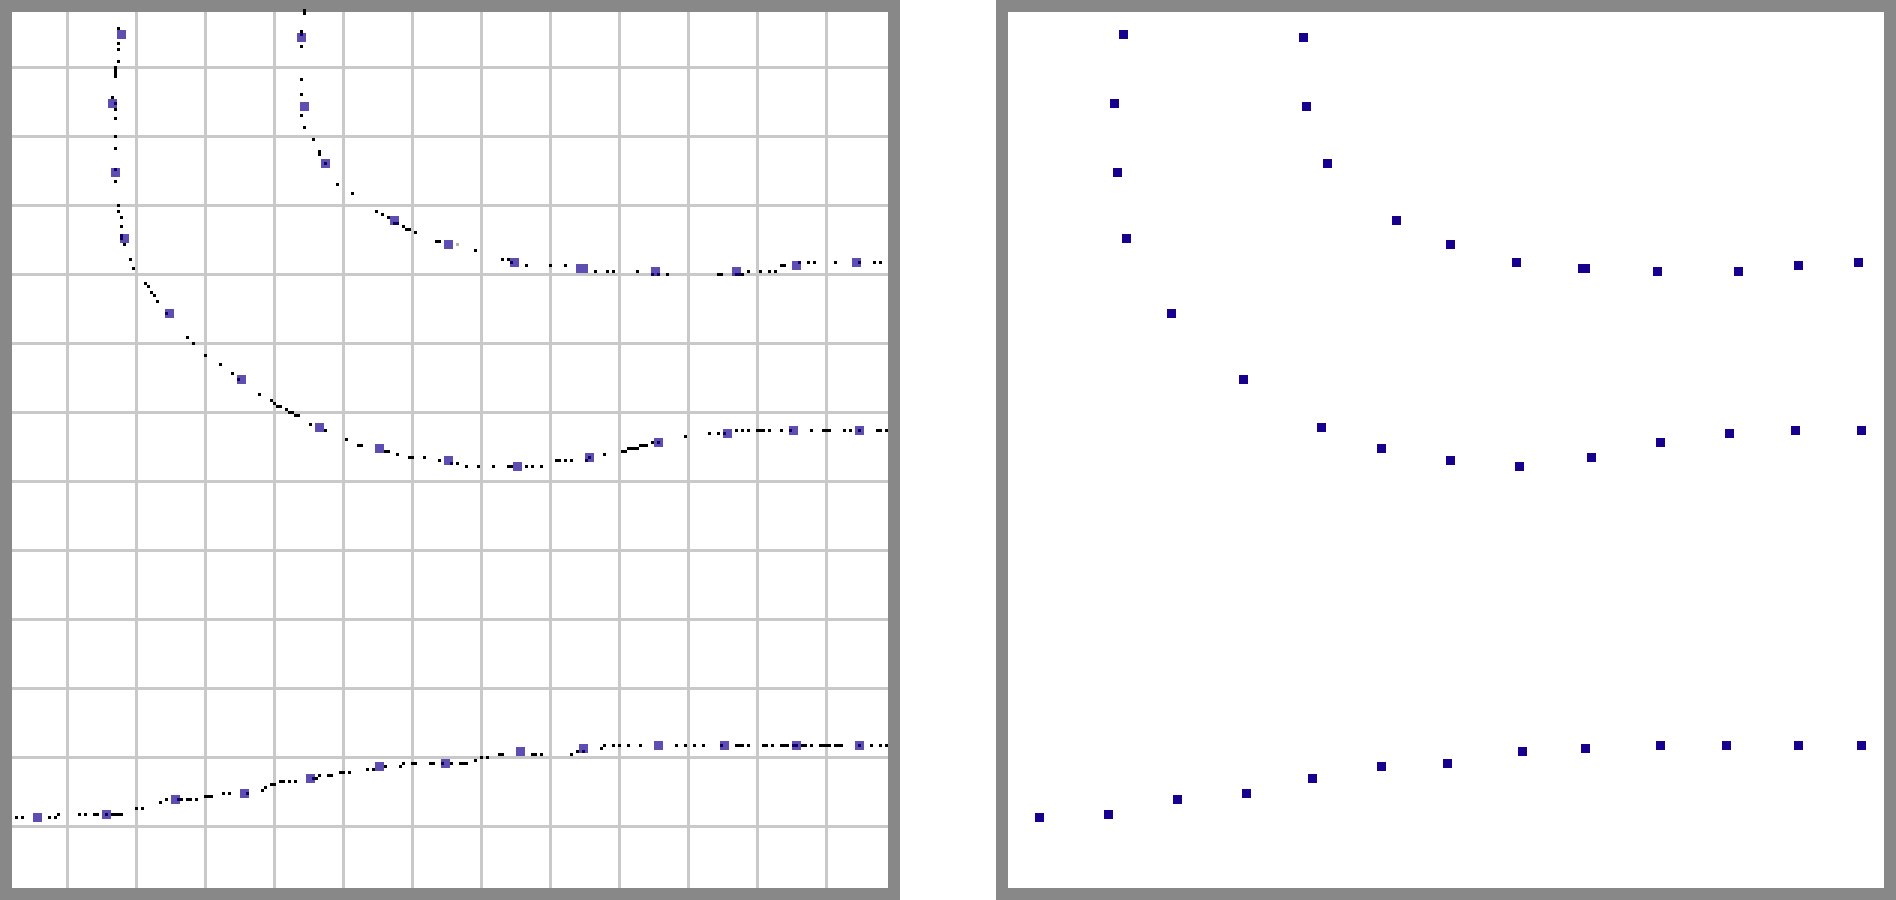
\includegraphics[width=7cm]{uniform.png}
\caption{Two-dimensional visualization of uniform downsampling algorithm}
\label{fig:uniform_algo}
\end{figure}

\begin{figure}[p]
\centering
\begin{gnuplot}
	set terminal epslatex color
	set xlabel "$l$"
	set ylabel "$n / |P|$"
	plot \
		"stat\_dragon.dat" using 1:($2/3609599+0*$2) smooth unique linetype rgb "black" title "dragon.ply", \
		"stat\_statuette.dat" using 1:($2/4999995+0*$2) smooth unique linetype rgb "red" title "statuette.ply", \
		"stat\_scan.dat" using 1:($2/681124+0*$2) smooth unique linetype rgb "blue" title "scan.ply"
\end{gnuplot}
\caption{Number of output points $n$ VS cubes side length $l$ in uniform downsampling}
\label{fig:uniform_stat}
\end{figure}

\begin{figure}[p]
\centering
\begin{gnuplot}
	unset key
	set ylabel "$n$"
	set xlabel "$s$"
	plot "uniform\_stat\_detail.dat" smooth unique
\end{gnuplot}
\caption{Close-up view of figure \ref{fig:uniform_stat}}
\label{fig:uniform_stat_detail}
\end{figure}


\subsection{Choosing the downsampling ratio}
The function $r(d)$ determines what ratio of downsampling that should be applied depending on the distance $d$ to the camera. If \emph{LOD regions} are used, it is a staircase function and can only take a small number of different values, otherwise (\emph{weighted points}) it is continuous. On what regions downsampling will be applied, and how $d$ is defined depends on the data structure used. (see next chapter.)

Let $L$ be the number of \emph{LOD regions} (``levels''). In the program, it is usually 1, 4, 8 or 16. For \emph{weighted points} downsampling, $L$ can take any value and can be changed at runtime. In both cases, $r(d)$ is defined the same way:

$r_{\ell}(\ell, a, L, n_{\text{total}}, n_{\min})$ gives the downsampling ratio for level $\ell \in [0, L-1]$. $n_{\text{total}}$ is the total number of points used as input to the downsampling algorithm, $n_{\min}$ the minimal number of points the should be outputted. If the algorithm is applied to the full model $n_{\text{total}} = |P|$ (number of points in model), and $n_{\min} = C$ (capacity of renderer) is used, since the goal is to stay as close as possible but inferior to $C$, so as to not lose more points than necessary. The function is defined such that $r_{\ell}(\ell = 0) = n_{\text{total}}$ (level 0 means no downsampling), $r_{\ell}(\ell = L-1) = n_{min}$ (maximal possible downsampling must be reached on last level), and it is stictly decreasing. The \emph{amount} parameter $a$ sets how strongly the function should be decreasing, and must be adjusted to fit the input model.

If \emph{LOD regions} are used, this function is evaluated during the preprocessing stage, when the $L-1$ downsampled point sets are created. For \emph{weighted points}, it is evaluated at runtime. Then, $a$ and $L$ also can be changed at runtime, and $\ell$ can take real values (as opposed to integers only). This allows for continuous downsampling.

The level to use at a given location is chosen by the function $\ell(d, s)$, where $d$ is the distance to the camera, and the \emph{setting} $s$ a parameter that can always be adjusted at runtime (unlike $a$). The function is defined such that $\ell(d = 0) = 0$ (no downsampling when very close to camera), and $\lim_{d \rightarrow \infty} = L-1$ (eventually reach maximal level). Also, it increases with $d$, where $s$ determines how quickly. $\ell(d, s)$ is defined as a real function, but when \emph{LOD regions} are used, the floor value $\lfloor \ell(d, s) \rfloor$ is always taken.

In short, the process of choosing the downsampling ratio $r(d)$ in function of distance $d$ works as follows: For \emph{weighted points}, $r(d) = r_{\ell}(\ell(d, s), a, L, n_{\text{total}}, n_{min})$ is evaluated at runtime, and $s, a, L$ can all be adjusted at runtime. Thus $r(d)$ is continuous.

For \emph{LOD regions}, $L$ point sets are created in the preprocessing stage which are downsampled with ratio $r_{ell}(i, a, L, n_{\text{total}}, n_{min})$. The integer $i \in 0 \hdots L-1$ is the level of the point set, and $a, L, n, n_{min}$ all need to be known in this stage. The program stores the downsampling ratios associated with the $L$ levels with the generated data structure. At runtime, the downsampled point set for level $i = \lfloor \ell(d, s) \rfloor$ is chosen depending on $d$. Only $s$ can be adjusted at runtime.

\subsection{Definition of the downsampling functions}
The downsampling level function $\ell$ is defined as follows:
\begin{displaymath}
	\ell(d, s) = \begin{cases}
		\min \{ \frac{d - d_{0}}{\Delta d}, L-1 \} & d > d_{0} \\
		0 & d \leq d_{0} \vee s = 0
	\end{cases}
\end{displaymath}

with $d_{0} = b^{1.3}$ the \emph{start distance}, i.e. the distance from the camera where downsampling should start, $\Delta d = b$ the \emph{step distance} after which the next level is chosen, and $b = \frac{250}{s}$.

So the level is chosen linearily with the distance, with an offset $d_{0}$. The \emph{setting} $s$ controls the intervals between levels and the start distance. The exponent $1.3$ for $d_{0}$ keeps $d_{0}$ larger than $\Delta d$, because the jump from no downsampling to the first level of downsampling represents a greater loss in output quality than a jump between downsampling levels.

The definition of $b$ makes sure $\ell(d)$ increases faster when $s$ is larger: If $s = 0$, $\ell$ is always zero, and no downsampling will be applied. If $d \gg 0$, eventually $\ell(d)$ will always yield the maximal downsampling level $L - 1$.

The following graph shows the function in its staircase form, with different values for $s$.

\begin{figure}[H]
\centering
\begin{gnuplot}
	set terminal epslatex color
	set ylabel "level"
	set xlabel "$d$"
	set ytics (0, 1, 2, 3, 4, 5, 6, 7, 8, 9, 10, 11, 12, 13, 14, 15)

	levels = 16
	xp = 1.3
	maxd = 700

	set xrange [0:maxd]
	set yrange [0:levels + 3]
	unset autoscale

	start_distance(b) = b**xp
	step_distance(b) = b
	constrain_lvl(l) = (l > levels - 1) ? (levels - 1) : l
	b(s) = 250 / s

	l(d, s) = constrain_lvl( \
		(d > start_distance(b(s))) ? ((d - start_distance(b(s))) / step_distance(b(s))) : 0 \
	)
	
	plot [d=0:maxd] \
		floor(l(d, 20)) with steps lt rgb "black" title "$s = 20$", \
		floor(l(d, 10)) with steps lt rgb "blue" title "$s = 10$", \
		floor(l(d, 50)) with steps lt rgb "red" title "$s = 50$"
\end{gnuplot}
\caption{Downsampling level for distance function $\ell(d, s)$}
\label{fig:downsampling_ell_d}
\end{figure}


The downsampling ratio function $r_{\ell}$ is defined as follows:
\begin{displaymath}
	r_{\ell}(\ell, a, L, n_{\text{total}}, n_{\min}) = 1 - (1 - r_{\min}) \left( \frac{\ell}{L-1} \right)^{a}
\end{displaymath}
where $r_{min} = \max \{ \frac{n_{\min}}{n_{\text{total}}}, 1 \}$ is the minimal downsampling ratio. Note that when $n_{\text{total}} \leq n_{min}$, the function always yields $1$ and no downsampling will be applied. 

The following graph shows the function with different values for the downsampling amount $a$:

\begin{figure}[H]
\centering
\begin{gnuplot}
	set terminal epslatex color
	set ylabel "$r$"
	set xlabel "level"
	set xtics (0, 1, 2, 3, 4, 5, 6, 7, 8, 9, 10, 11, 12, 13, 14, 15)

	n = 5000000
	nmin = 1000000
	rmin = nmin / n
	levels = 16

	set xrange [0:(levels - 1)]
	set yrange [0:1]
	unset autoscale
	
	r(l, a) = 1 - (1 - rmin) * (l/(levels - 1))**a
	plot [l=0:(levels - 1)] \
		r(l, 2) lt rgb "black" title "$a = 2.0$", \
		r(l, 1.2) lt rgb "blue" title "$a = 1.2$", \
		r(l, 0.4) lt rgb "green" title "$a = 0.4$", \
		r(l, 3.8) lt rgb "red" title "$a = 3.8$"
\end{gnuplot}
\caption{Downsampling ratio function $r_{\ell}(d, a)$}
\label{fig:downsampling_r_ell}
\end{figure}

\begin{wrapfigure}{r}{7cm}
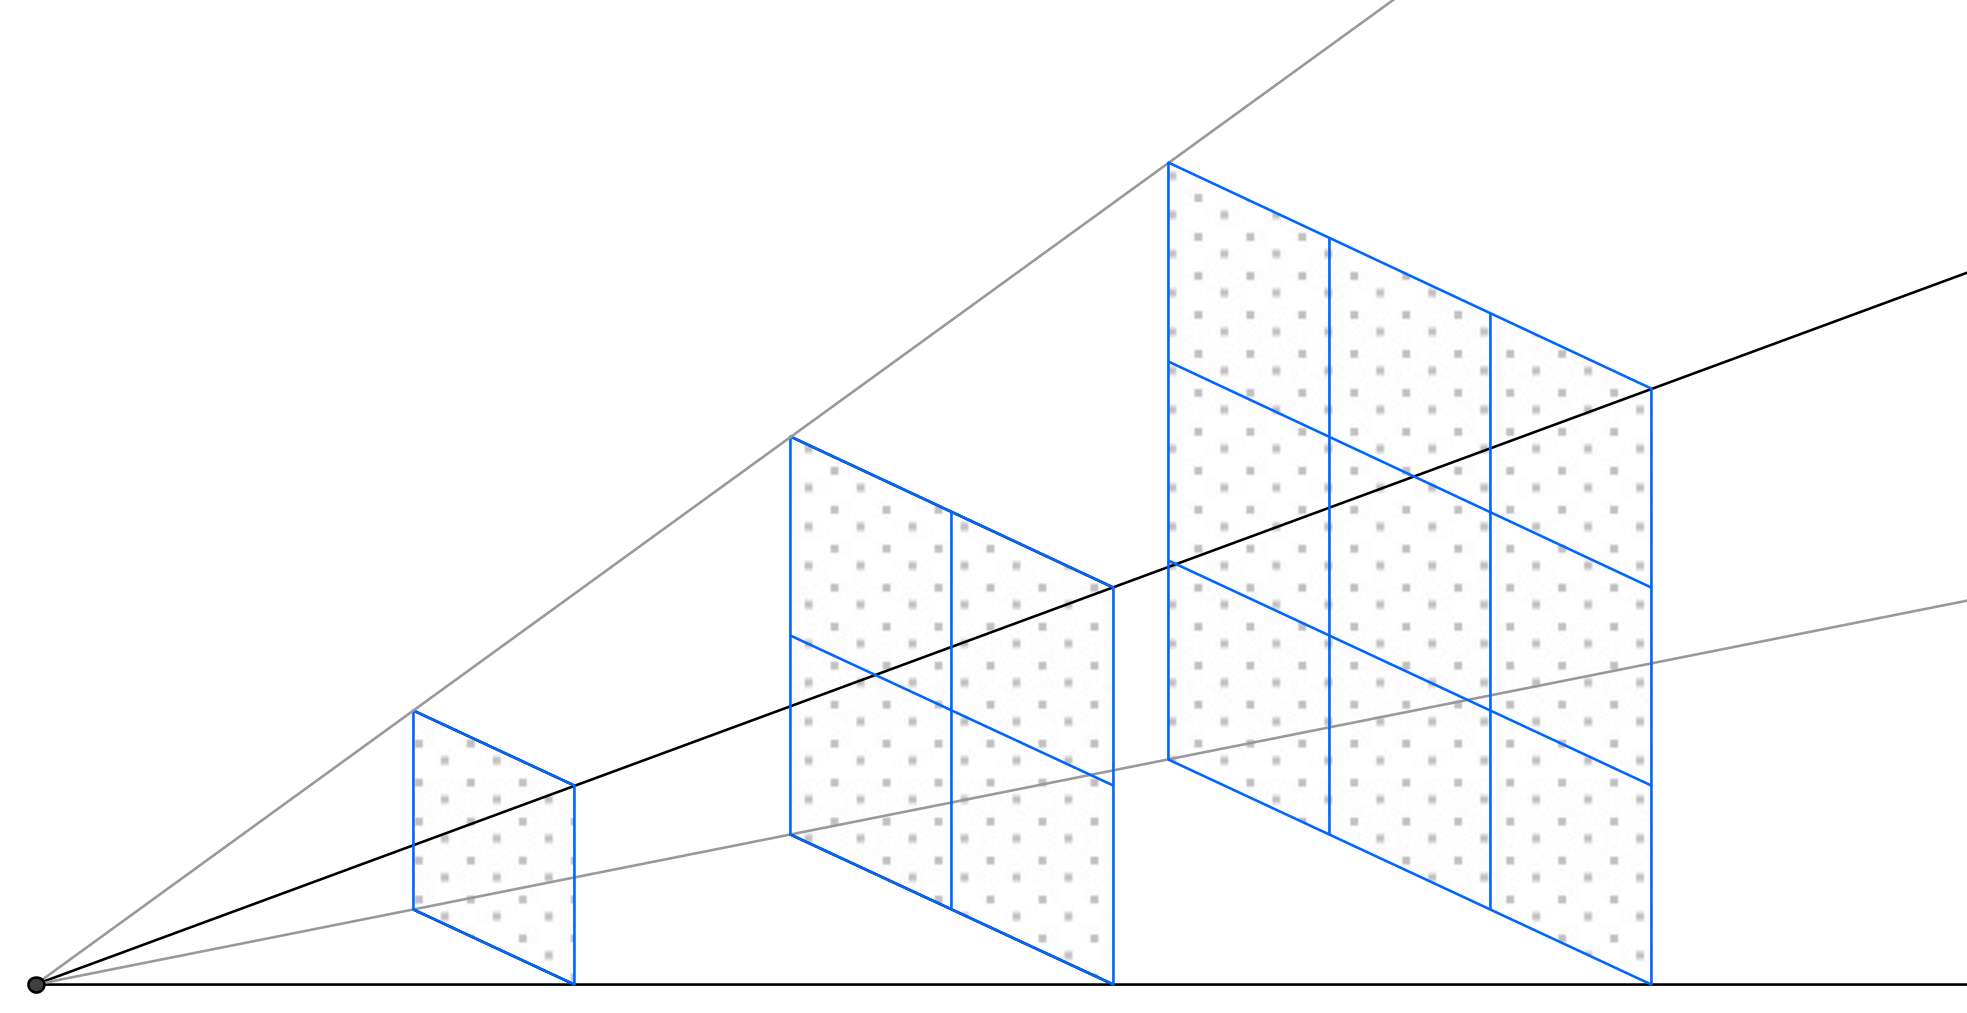
\includegraphics[width=7cm]{distanceDensity.png}
\caption{Perspective projection and area}
\label{fig:distance_density}
\end{wrapfigure}
Figure \ref{fig:distance_density} shows visible areas\footnote{In reality, the areas would be curved (intersection of view frustum and sphere of radius $d$), but the simplification holds because the field of view is small} with distances $d$, $2d$ and $3d$ to the camera in a perspective projection. Their area is proportional to $d^{2}$. Supposing that surfaces of the point cloud is located exactly on these areas, the point density of the projection $\rho'$ would also be proportional to $d^{2}$.

Since $\rho'$ should be more or less constant, setting $a = 2$ makes sense as it cancels out the effect. In practice, it needs to be adjusted to fit the particular point cloud.

Finally, this graph shows $r_{d, s}$ ($r_{\ell} \circ \ell$) in piecewise form, with $a = 2$, $L = 16$ and $r_{\min} = 0.2$:

\begin{figure}[H]
\centering
\begin{gnuplot}
	set terminal epslatex color
	set ylabel "$r$"
	set xlabel "$d$"

	levels = 16
	xp = 1.3
	maxd = 800
	n = 5000000
	nmin = 1000000
	rmin = nmin / n
	a = 2
	b(s) = 250 / s

	start_distance(s) = b(s)**xp
	step_distance(s) = b(s)
	constrain_lvl(l) = (l > levels - 1) ? (levels - 1) : l

	r(l) = 1 - (1 - rmin) * (l/(levels - 1))**a

	l(d, s) = constrain_lvl( \
		(d > start_distance(s)) ? ((d - start_distance(s)) / step_distance(s)) : 0 \
	)
	
	rd(d, s) = r( 0.0 + floor( l(d, s) ) )
	rdc(d, s) = r( 0.0 + l(d, s) )
	
	plot [d=0:maxd] \
		rd(d, 20) with steps lt rgb "black" title "$s = 20$", \
		rd(d, 10) with steps lt rgb "blue" title "$s = 10$", \
		rd(d, 50) with steps lt rgb "red" title "$s = 50$"
\end{gnuplot}
\caption{Downsampling ratio for distance $r(d, s)$}
\label{fig:downsampling_r}
\end{figure}

\subsection{Effect of downsampling setting}
The following graph shows how the downsampling setting $s$ affects the number of outputted points $n$, on different camera view points and for different models. Since downsampling is applied on the point set that was already filtered by view frustum culling, the camera position and orientation have a great effect on the output range.

\begin{figure}[H]
\centering
\begin{gnuplot}
	set terminal epslatex color
	set xlabel "$s$"
	set ylabel "$n / n_{\min}$"
	set yrange [0.0:1.1]

	nmin = 1000000
	plot \
		"setting\_output\_stat/statuette\_inside\_cm8.dat" using 1:($2/nmin+0*$2) smooth unique title "statuette inside cm8", \
		"setting\_output\_stat/statuette\_far\_cm8.dat" using 1:($2/nmin+0*$2) smooth unique title "statuette far cm8", \
		"setting\_output\_stat/dragon\_inside\_cm8.dat" using 1:($2/nmin+0*$2) smooth unique title "dragon inside cm8", \
		"setting\_output\_stat/dragon\_inside\_c.dat" using 1:($2/nmin+0*$2) smooth unique title "dragon inside c", \
		"setting\_output\_stat/dragon\_closeup\_cm8.dat" using 1:($2/nmin+0*$2) smooth unique title "dragon closeup cm8"
\end{gnuplot}
\caption{Number of output points $n$ on downsampling VS downsampling setting $s$}
\label{fig:uniform_stat}
\end{figure}

The outputted number of points $n$ never gets larger than $n_{\min}$ because in this example $n_{\min} = C$ the capacity of the renderer, and the algorithm that extracts points from the data source never outputs more than $C$ points. It is chosen so that in the extreme case where all points from $P$ lie in the view frustum, it can still be rendered by choosing the highest downsampling level $\ell = L-1$ everywhere. This is the case in \texttt{dragon far cm8}. frustum culling makes the actual outputted number of points $n$ smaller than $n_{\min}$ as seen in the graph.

For viewpoints where only a small portion of the model is visible, $n$ can remain smaller than $n_{min}$ for any setting. An extreme case is a close-up view as shown in \texttt{dragon closeup cm8}.

The optimal setting $s$ is one where $n$ is as large as possible, but below $n_{min}$. If it is smaller than it could be, the renderer capacity would still allow for a higher number of points and thus higher quality. If it hits $n_{min}$, then the program attempts to extract more than $C$ points and breaks up in the process, leading to missing parts in the output.

Also the aspect of the curve varies greatly with the camera position and orientation, especially for composite models where different parts have different point densities. So the user would have to keep adjusting the setting $s$ in order to get good results. It may be possible to implement a controller mechanism that automatically adjusts $s$. Possibly a system similar to a \emph{PID} controller could be used. This is not implemented in the program.




\section{Occlusion culling}
Occlusion culling, or hidden surface removal is the process of removing points from $P$ that are occluded by another points surface in front of it. The algorithms have no knowledge about the shape of the surfaces, but only operate on the assumption that the model is such that all points lie on a surface with a density $\rho$ that remains locally more or less constant. Removing the occluded points aids in reducing the size of $P'$, and also makes the output look better.

Different algorithms exist to approximate occlusion culling on a point set without knowledge of the surfaces.

\subsection{Point shadows}
A simple method that is implemented in the application is do draw a black \emph{shadow} behind each rendered point. The shadow is a disk or square a few pixels wide centered around the point. If a surface is at a reasonable distance from the camera, its points will all be just a few pixels apart on the projection, and the shadows completely cover the points behind it. Thanks to the GPU's \emph{depth testing}, this still works when those points are rendered after the ones from the occluding surface.

The method can improve visual quality, but it no longer works when the camera is too close to the surface, and as a side effect it produces black contours around the edges of the model, since the shadows don't take the (unknown) normal vectors of the points on their surface into account. Also, it increases the load on the GPU too much since every pixel of the shadow is processed the same way as a point from $P'$, and there can easily be many unnecessary overlapping pixels. Because it is implemented on the GPU (as an OpenGL shader), it does not contribute to the goal of reducing the size $P'$ to fit $C$.

\subsection{HPR Operator}
Another possibility is the \emph{HPR operator} described in \cite{Kat2007}: In a coordinate system centered around the current camera position $O$, the following \emph{spherical flipping} transformation is applied to the points in the view frustum:
\begin{equation}
	p' = p + 2(R - |p|) \frac{p}{|p|}
\end{equation}

where $R$ is the radius of a sphere centered in $O$ that covers all visible points. This transformation has the property that if for two points $p_{1}, p_{2}$, one has that $p_{1}$ is closer to $O$ than $p_{2}$, then the image $p'_{1}$ will now be further away from $O$ than $p'_{2}$.

Then, the convex hull is calculated on the transformed point set. As output, the algorithm returns only the points $p \in P$ whose image $p'$ is part of that convex hull. The following picture illustrates the transformation in 2D, along with the resulting output. The figure is copied from \cite{Kat2007}.

\begin{figure}[H]
\centering
	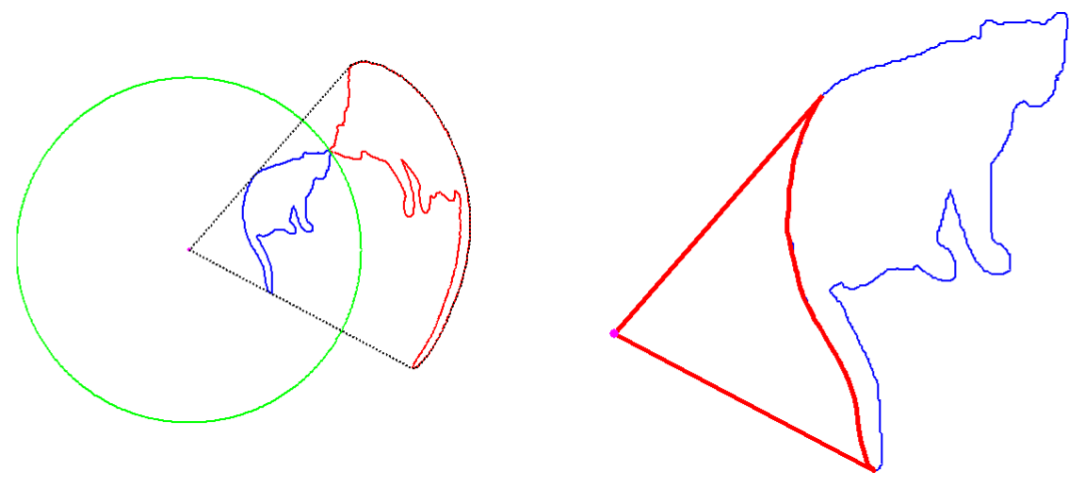
\includegraphics[width=10cm]{hpr.png}
\end{figure}

However, this algorithm is not usable in a dynamic setting because of the complexity of computing the three-dimensional convex hull of a large point set. It tends to take a few seconds for about $3000$ points.

An modified ``Fast HPR operator'' is presented in \cite{Ren2012} that calculates an approximate convex hull instead. According to the article, this technique may be efficient enough for interactive usage.

In short, it works in a manner similar to uniform downsampling. The view frustum is subdivided into a regular grid of three-dimensional sectors pointing outward the camera into the visible points. For each sector only the point furthest away is retained.\footnote{Actually the dot product of the point with the directing vector at the center of the sector is compared.} Then the algorithm applies additional post-processing on neighboring sectors to improve the quality of the convex hull approximation.



\chapter{Data structures}
The $f_{P}$ function described in the previous chapter takes a unordered set $P$ of three-dimensional points as input. In an implementation, $P$ will be stored in a certain \emph{data structure}, which itself exists as a one-dimensional array of bits. The data structure will hold the points $P$, along with weights or \emph{LOD} sets for downsampling, and possibly additional information. The criterion for choosing a data structure is that $f_{P}$ can be implemented in an efficient way.

\section{General}
Since the data structure must contain all the $n_{\text{total}}$ points of $P$, its size must always be at least in $O(n_{\text{total}})$. The algorithm which extracts $P' = f_{P}$ will typically only need to read a small portion consisting of $n \ll n_{\text{total}}$ points. To make this efficient the data structure must be designed such that:
\begin{itemize}
\item It must be possible to determine the portions of data to extract without searching through the whole structure. The worst case would be a data structure that consists simply of an array of points in any order, because to find the points that lie inside the current view frustum the algorithm would have to check every point in the array, leading to a time complexity $O(n_{\text{total}})$.
\item The data structure is always serialized to storage in one dimension. It is generally much more efficient to read a small number of long segments, rather than many small segments: Seeking times on the storage device are avoided, and various caching mechanisms from the underlying file system take effect.

No order can be defined for three dimensional points, but their one-dimensional representations always have an order. So a compromise needs to be found by which the serialization is ordered such that for the majority of cases, points that are close to each other in three dimensional space remain close to each other in the serialization.
\end{itemize}

Two techniques are used to achieve this: The model is split into smaller \emph{regions}, and the points within that region remain grouped together in the data structure. Points within the same regions have the property that their distance is upper bounded by the size of the region, and so this contributes to the ordering issue. Also, \emph{pointers} is used in various ways, meaning reading algorithm will directly jump to a given offset in the data independently of its distance.

\section{File types}
The data structure is built on top of a \emph{file type}. Several possible file types were compared:
\begin{description}
\item[Raw file] Essentially no file type is used, and the data structure is implemented on the lowest level. The implementation needs to write and read the structure as a single continguous segment of binary data. This allows for the highest level of control, but requires an ad-hoc definition of helper structures such as a way to split the file into different parts for points, downsampled points, regions, additional file information... Also the precise way that data values serialized (floating point and integer data types, alignment, endianess) needs to be taken care of in the implementation of the data structure.
\item[ASCII-based file] Storing data as an ASCII-based text file instead of as raw binary data removes the latter problems of data serialization. The remaining problems stay the same. The files get much larger: If the file contains a set of $1000000$ points with $x, y, z$ coordinates, storing them as 4 byte floating point values would require $\SI{11.72}{\mega\byte}$. If the values are written in decimal representation with 8 digits, plus separation characters, a size of about $\SI{29.56}{\mega\byte}$ would result. This additional space requirement, and the parsing overhead when reading from the file, makes such file types impractical for large amounts of data.
\item[XML] XML would provide a way to represent structured data, and so it would be possible to build the data structure in terms of XML tags, containers and attributes. However, it suffers the same problems as any ASCII-based format, to an increased extent since it tends to be very verbose compared to simpler formats. Also, the purpose of XML is not to deal with large amounts of data that is dynamically read, but rather to deal with relatively small, deeply structured files such as computer programs or web pages, and it provides tools to validate, transform, interlink, etc. such files.
\item[HDF] HDF (\emph{Hierarchical Data Format}) is the main format used in the program. It is a binary format designed for storage of large quantities or scientific data in such a way that parts of it can be extracted efficiently. It stores the data sets either directly as sequential data on the storage device, but can also internally store the data sets in multiple chunks, and provide additional optimizations such as internal caches for dealing with large data sets.
\item[SQL database] Using a relational database such as \emph{SQLite} allows for implementing the structure on a higher level, while the database takes care of arranging the data internally so as to allow for fast retrieval. This includes its internal data structures and algorithms used to implement indexing, executing \emph{SELECT} queries, caching...
\end{description}

In general, it seems a much better choice to stay with a lower level file format like \emph{HDF} that still provides basic facilities for separating data sets, defining data types, etc. The definition of the \emph{data structure} should include how it is serialized to a one-dimensional representation, since this is critical for its performance.

\section{HDF}
The \emph{Hierarchical Data Format} HDF, was designed to allow for storing large quantities of multi-dimensional numerical data, such as fields recorded by scientific instruments. Using it to serialize a data structure is not its main purpose, but the features \emph{HDF} provides still make it a good choice. Here is a brief overview of some building blocks of \emph{HDF5}:
\begin{description}
\item[data type] Usually numeric (integer or real), possible to have fixed length arrays for any data type. The precise representation (endianness, bit size) can be defined.
\item[combound data type] Similar to a \texttt{struct} in C: Data type composed of several named members of different types.
\item[data set] An HDF5 file contains one or more data sets, and these contain the actual data. It has a data type (can be combound), and can be one- or multi-dimensional. Usually its length needs to be specified at creation, but \emph{chunked data sets} are stored internally in a way that allows for a dynamic unlimited extend.
\item[data space] A selection of data in a data set. Can be a simple one-dimensional interval, or a \emph{hyperslab} that can represent a selection on a serialized multi-dimensional data set. Data is read and written into data spaces.
\item[attribute] Single named data values that can be attributed to a data set or another object. Used to attach additional information to the file.
\end{description}
Here, only one-dimensional data sets are used. The \texttt{points} data set would be a data set of a combound type \emph{point}, which has data members for the coordinates and color.

\section{Cuboid regions} \label{sec:cub_reg}
All of the data structures used in the projet rely on subdividing the three dimensional space in axis-aligned cuboid regions. A cuboid $\mathcal{C}$ is defined by its \emph{origin} $(x, y, z)$ and its \emph{extremity} $(x', y', z')$, and a point $\overrightarrow{p}$ is considered to be inside the cuboid if and only if $p_{x} \in [x, x'[$, $p_{y} \in [y, y'[$ and $p_{z} \in [z, z'[$.

Because the intervals are open on one side, points that lie on the border of two adjacent cuboids can never fall into both of them. However, when defining a bounding cuboid that should enclose a given set of points, it becomes necessary to make the coordinates of its extremity slightly larger than the point with maximal coordinates.

\subsection{Floating point issues}
Cuboids are defined in terms of origin and extremity, instead of origin and side lengths, in order to deal with floating point imprecision problems that would otherwise occur in the implementation: For the \emph{tree structures}, cuboids will be recursively subdivided into smaller cuboids, out of which some share extremity coordinates with the parent cuboid. If side lengths were to be used, those floating point values would not be copied, but rather need to be recomputed from the new origins and side lengths of the child cuboids. This will make their values slightly different, and as a consequence the algorithms would be incorrect. They could for instance encounter points that are inside a child cuboid, but outside the parent cuboid.
These edge cases are significant because the coordinates are real values, whereas quantities of points are discrete. Parts of the program rely on having exact knowledge of these quantities, for example to align data segments in files the right way.

In other situations where floating point imprecisions are tolerated, the program uses a small threshold value $\epsilon$ to test two floating point values for ``equality''. That is, $f_{1} \approx f_{2} \Longleftrightarrow |f_{1} - f_{2}| < \epsilon$.

\subsection{Point-to-cuboid distance}
Also for all of the data structures, the implementation of $f_{P}$ will apply downsampling to entire cuboid regions with a constant downsampling ration $r$. This ratio is determined by $r(d, s)$ as described in the previous chapter, where $d(\overrightarrow{p}, \mathcal{C})$ is a \emph{point-to-cuboid distance} from the camera position to the cuboid. The program allows the user to choose between several definitions for $d$:
\begin{description}
\item[center] The distance from $\overrightarrow{p}$ to the centroid $( \frac{x + x'}{2}, \frac{y + y'}{2}, \frac{z + z'}{2} )$ of $\mathcal{C}$.
\item[minimal] The minimal distance from $\overrightarrow{p}$ to any position $\overrightarrow{q}$ on the border of $\mathcal{C}$. The $\overrightarrow{q}$ which gives the minimal distance may be a corner of $\mathcal{C}$, or an orthogonal projection of $\overrightarrow{p}$ on either an edge or a side of $\mathcal{C}$.
\item[maximal] The maximal distance from $\overrightarrow{p}$ to any position $\overrightarrow{q}$ on the border of $\mathcal{C}$. In this case, $\overrightarrow{q}$ is always a corner of $\mathcal{C}$.
\item[mean] The mean value of the minimal and maximal distances.
\end{description}

\begin{wrapfigure}{r}{4cm}
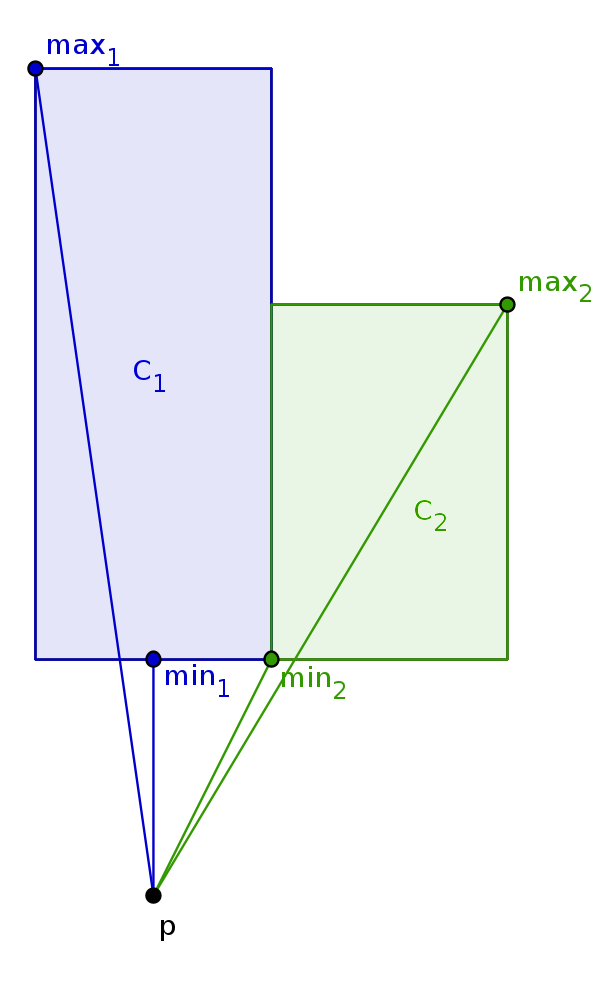
\includegraphics[width=4cm,height=5cm]{minMaxDistance.png}
\label{fig:min_max_c_d}
\end{wrapfigure}
Assuming that any definition of $d$ gives a value $\geq$ the maximal distance and $\leq$ the minimal distance, it is not possible in general to define $d$ such that if $d(\overrightarrow{p}, \mathcal{C_{1}}) > d(\overrightarrow{p}, \mathcal{C_{2}})$, then for all $\overrightarrow{q_{1}} \in \mathcal{C_{1}}$ and all $\overrightarrow{q_{2}} \in \mathcal{C_{2}}$, it remains true that $d(\overrightarrow{p}, \overrightarrow{q_{1}}) > d(\overrightarrow{p}, \overrightarrow{q_{2}})$. 

The figure on the right illustrates this: $d(p, \min_{1}) < d(p, \min_{2})$, whereas $d(p, \max_{1}) > d(p, \max_{2})$. So no matter how the \emph{point-to-cuboid distance} is defined in that case, there will always be points in one of the cuboids that don't fullfill the condition. When such points are inside the view frustum, is leads to visual discontinuities, as there are places where the downsampling ratio gets lower at a greater distance instead of higher.

As a compromise, one of the proposed definitions needs to be chosen chosen that reduces this effect. Generally, better results are produced when the regions are more or less cubic, and in that case the \textbf{center} definition of $d$ yields good results. Otherwise, \textbf{minimal} tends to be better.

\pagebreak

\section{Cubes structure}
The \emph{cubes structure} is a first attempt at a simple way to organize the set of points such that the algorithm is faster than a naive implementation that would iterate through the whole set of points at each evaluation of $f_{P}$.

Space is subdivided into a regular grid of axis-aligned \emph{cubes} $\mathcal{C}_{i,j,k}$ with a common side length $l$.\footnote{This is unrelated to the cubes used for uniform downsampling in the previous chapter.} These cubes are the cuboid regions for this structure. Because of the way their boundaries are defined, every point $p \in P$ will belong into exactly one cube. The side length can be configured when the structure is created, and is by default set to $l = 5$. The integers $i, j, k$ are the coordinate indexes for the cubes in the grid. For the cube $\mathcal{C}_{0,0,0}$, its \emph{origin} corresponds to the origin of the space.

Only cubes that contain at least one point are created, so their total number will be finite. In the first stage of the structure creation progress, the algorithm iterates through the full set of points $P$, and for each point $p$ determines the coordinates of the cube into which $p$ will belong by floor division:
\begin{equation*}
	(i, j, k) = \left( \lfloor p_{x}/l \rfloor, \lfloor p_{y}/l \rfloor, \lfloor p_{z}/l \rfloor \right)
\end{equation*}
This is correct because the definition of the floor function coincides with the way that the cuboid regions' boundary intervals are defined. Similar relations will occur for the tree structures, where it is critical for the correct functionning of the algorithm that the relations always hold, despite possible floating point imprecision errors.

There are two variants for the cubes structure, one with \emph{weighted points} and one with \emph{LOD regions}. 

\subsection{Weighted point variant}
The algorithm proceeds by attributing random weights $w \in [0,1]$ to each point $p \in P$ in an uniform distribution.

When a \emph{HDF} file type is used, two one-dimensional data sets \texttt{points} and \texttt{cubes} are created. The \texttt{points} data set contains $|P|$ entries of the \texttt{point} compound type. This type consists of four floating point values for the point coordinates $p_{x}, p_{y}, p_{z}$ and the weight $w$, plus three byte values for the RGB color information. The points in $P$ are added into this data set, grouped by the cube in which they belong. Inside each cube group, the point entries are sorted by ascending $w$. The outer order of the cube groups does not matter.

The \texttt{cubes} data set is filled with an entry for each cube. For each cube entry, it contains the three indexes of the cube $i, j, k$, the number of points in the cube $N(\mathcal{C})$, and the offset $\text{off}(\mathcal{C})$ in the \texttt{points} data set of the first point from that cube. So in given a \texttt{cubes} entry the corresponding array of points in \texttt{points} ranges from $\text{off}(\mathcal{C})$ to $\text{off}(\mathcal{C}) + N(\mathcal{C}) - 1$.

This data structure is also implemented with an \emph{SQLite database} as backend. Here, two tables for the cubes and for the points are created, except that instead of storing offsets, each cube gets a unique \emph{primary index} and, the points table contains an \emph{foreign key index} column that is set to its cube's index. The points corresponding to one cube are loaded using SQL queries, and \emph{SQLite}'s indexing algorithms take care of the internal representation of the data and then necessary optimizations.

\subsection{LOD regions variant}
For the \emph{LOD regions variant}, the algorithm instead proceeds by generating, for the sets of points in each cube $P_{\mathcal{C}} = \{ p \mid p \in \mathcal{C} \}$, the $L-1$ downsampled point sets $P'_{r}(\mathcal{C})$.\footnote{An alternative implementation would be a generate the downsampled point sets for the entire model $P$, and then reattribute the resulting points $p' \in P'_{r}$ to their respective cubes.}

In the \emph{HDF} file, $L$ different point sets \texttt{points\#} are created which will be filled with all the points for the downsampled point sets. Again, the points are grouped by their cube. Here, the points don't have a weight, and the order of the point entries inside the groups, just like the order of the groups, does not matter. The \texttt{cubes} data set now needs to store the cubes' point offsets and counts for each downsampling level, because they will be different.

There is no implementation for a \emph{SQLite database} file type for this variant.


\subsection{Extraction algorithm}
The \emph{extraction algorithm} of a data structure is executed repeatedly as the user moves through the point cloud and his camera position and view frustum changes. One of the main goals of the project is for this algorithm do be as efficient as possible, even when the model is very large.

For the cubes structure, the algorithm iterates through the full list of cubes each time, and for each cube, checks whether it is completely or partially inside the view frustum. This test is done on the cube alone and without considering the points in that cube, using the test described in \ref{sec:fr_cub_inter}. If the test is positive, it determines a downsampling level $\ell$ for that cube using $\ell(d, s)$ where the point-to-cuboid $d$ is calculated by one of the schemes described above.

For the \emph{LOD regions} variant, it then copies the all of the points of the cube for level $\ell$ from the file into the output buffer. This always a single segment of data. For the \emph{weighted points} variant, it extracts the points for which $w < r$. So this requires iterating through the points, but because the points are sorted by ascending $w$, the procedure can stop when $w \geq r$ is reached. So the \emph{weighted points} variant is slower, but requires less storage space. It also allows for $r$ of a cube to take any value as opposed to only $L$ possibilities. But small discontinuities still occur at the boundaries of the cubes grid.

The complexity of the algorithm is linear with respect to the number of cubes, and so it scales too much with the size of the model.

\pagebreak

\section{Tree structures}
The \emph{tree structures} recursively subdivide space into cuboid regions. A \emph{root cuboid} is taken that encloses the entire model\footnote{Due to the definition of the cuboid boudaries, its extremity coordinates need to be made slightly larger than the maximal point coordinates.} Then, according to a certain rule, that cuboid is subdivided into $c$ \emph{child} cuboids. These child cuboids must be such that they don't overlap, don't go outside the original (\emph{parent}) cuboid, and completely cover the \emph{parent} cuboid. This process is recursively repeated, until the number of points $p$ that lie inside a cuboid $\mathcal{C}$ is smaller or equal to the \emph{leaf capacity} $k$. These cuboids are the \emph{leaves} of the tree formed by the hierarchy of cuboids.


\section{Serialization} \label{sec:tree_ser}
The constraints for the rule by which the cuboids are subdivided imply that it is possible to order the points in such a way that the subset of points inside a given cuboid $\mathcal{C}$ of any depth always lie on one segment of the ordered list.

If $\mathcal{C}_{1}$ is a child cuboid of $\mathcal{C}_{0}$, then $p \in \mathcal{C}_{1} \Rightarrow p \in \mathcal{C}_{0}$, and if $p \in \mathcal{C}$ and $\mathcal{C}$ is not a leaf, there must exist exactly one child cuboid of $\mathcal{C}$ that also contains $p$. This relation can be reproduced in the one dimensional representation by recursively subdividing segments in the same manner. So, each cuboid will be associated an \emph{offset} $\text{off}(\mathcal{C})$ in the points list, and a \emph{number of points} $N(\mathcal{C})$.

Just like with the \emph{cubes structure}, downsampling can be added through the use of \emph{LOD regions}. However, it is no longer possible to effectively implement a \emph{weighted points} variant: The points belonging to a cuboid cannot be ordered by their weight $w$ because subsegments would also have to be ordered the same way. Without this, the program would be forced to iterate through all points in the view frustum.

Similarly to cubes in the \emph{cubes structure}, cuboids ``nodes'' are stored in a separate list, with their link (offset, count) to the points sets. Also the offsets (in the same list) of a node's child nodes are stored with it, as well as the node's cuboid. There is no need for the nodes to be ordered in a specific way.\footnote{This is useful in a parallelized implementation of the structure creation algorithm; see further.} Storing the cuboid with the node slightly increases the file size, but it simplifies implementation, and allows for trees formed by several different rules. (see later)

In the implementation, \emph{splitters} define the rule by which the cuboids are chosen and subdivided. The following three are implemented:

\subsection{Octree}
All cuboids must be cubic, i.e. have equal side length. The \emph{root cuboid} will be the smallest cube that encloses the entire model, such that the model is placed at the center of that cube. Each cube will be subdivided into 8 child cubes, that are on the 8 sides of the cube's center point.

This is a good option in most cases because the regions are cubic, and so choosing the distance from the camera to the center of a cube as \emph{point-to-cuboid} distance yields good results.

\subsection{KdTree}
For the \emph{KdTree}, the cuboids no longer need to be cubes. Each cuboid is split into 2 child cuboids. The \emph{split plane} that separates them is alternately orthogonal to the $X, Y, Z, X, ...$ axis, depending on the \emph{depth}\footnote{The \emph{depth} of the \emph{root cuboid} is set to 0. For each cuboid $\mathcal{C}$, its depth is that of its parent plus one.} of the cuboid modulo 3. Two different ways of choosing the position of the split plane on that axis are implemented:

\subsubsection{Half}
The split plane is always at the center of the cuboid. That way if the \emph{root cuboid} is near-cubic, child cuboids won't diverge from a near-cubic shape. Its advantage over the \emph{Octree} is that there are only two children per node, which useful for the \emph{piecewise tree structure} (see further).

\subsubsection{Median}
In the proper definition of a \emph{KdTree}, the position of the \emph{split plane} is at the median of the coordinates for the given axis, of all the points in the cuboid. This implies that there will be the same number of points in both children, and so the entire tree will be perfectly balanced.

This could in general accelerate descent into a tree. But it does not present an advantage here, and leads to two problems: The cuboids tend to become strongly non-cubic, making it impossible to define a good \emph{point-to-cuboid distance}. And in order to calculate the median, the entire array of coordinates needs to be stored temporarily in memory and then sorted. This is not practical for large point sets.

There are algorithms for approximating a median value without this. For example, one way would be to build a histogram on intervals, find its median, and repeat the same on that interval. This is not implemented in the application.

\subsection{Splitter}
The \emph{splitter} of a \emph{tree structure} consists of these elements:
\begin{description}
\item[adjust root cuboid] For example making the root cuboid cubic for the \emph{OcTree}.
\item[node points information] Information associated to each node that is deduced from the points in the cuboid. For \emph{KdTree}, it is the position of the split plane.
\item[child cuboid function] Calculates the cuboid of a child node, using the child index $i$, the \emph{node points information}, and the \emph{depth} and \emph{cuboid} of this node.
\item[child index function] Calculates the index of the child (of this node) that contains a given point $p$. Also uses the \emph{node points information}, \emph{depth} and \emph{cuboid} of this node. This can be implemented more simply than checking every child cuboid, for example using just a floating point value comparison with the \emph{KdTree} \emph{split plane} position.
\end{description}
As described previously, the implementation must take care of floating point imprecisions for these two functions.

\subsection{Extraction algorithm}
\begin{wrapfigure}{r}{6cm}
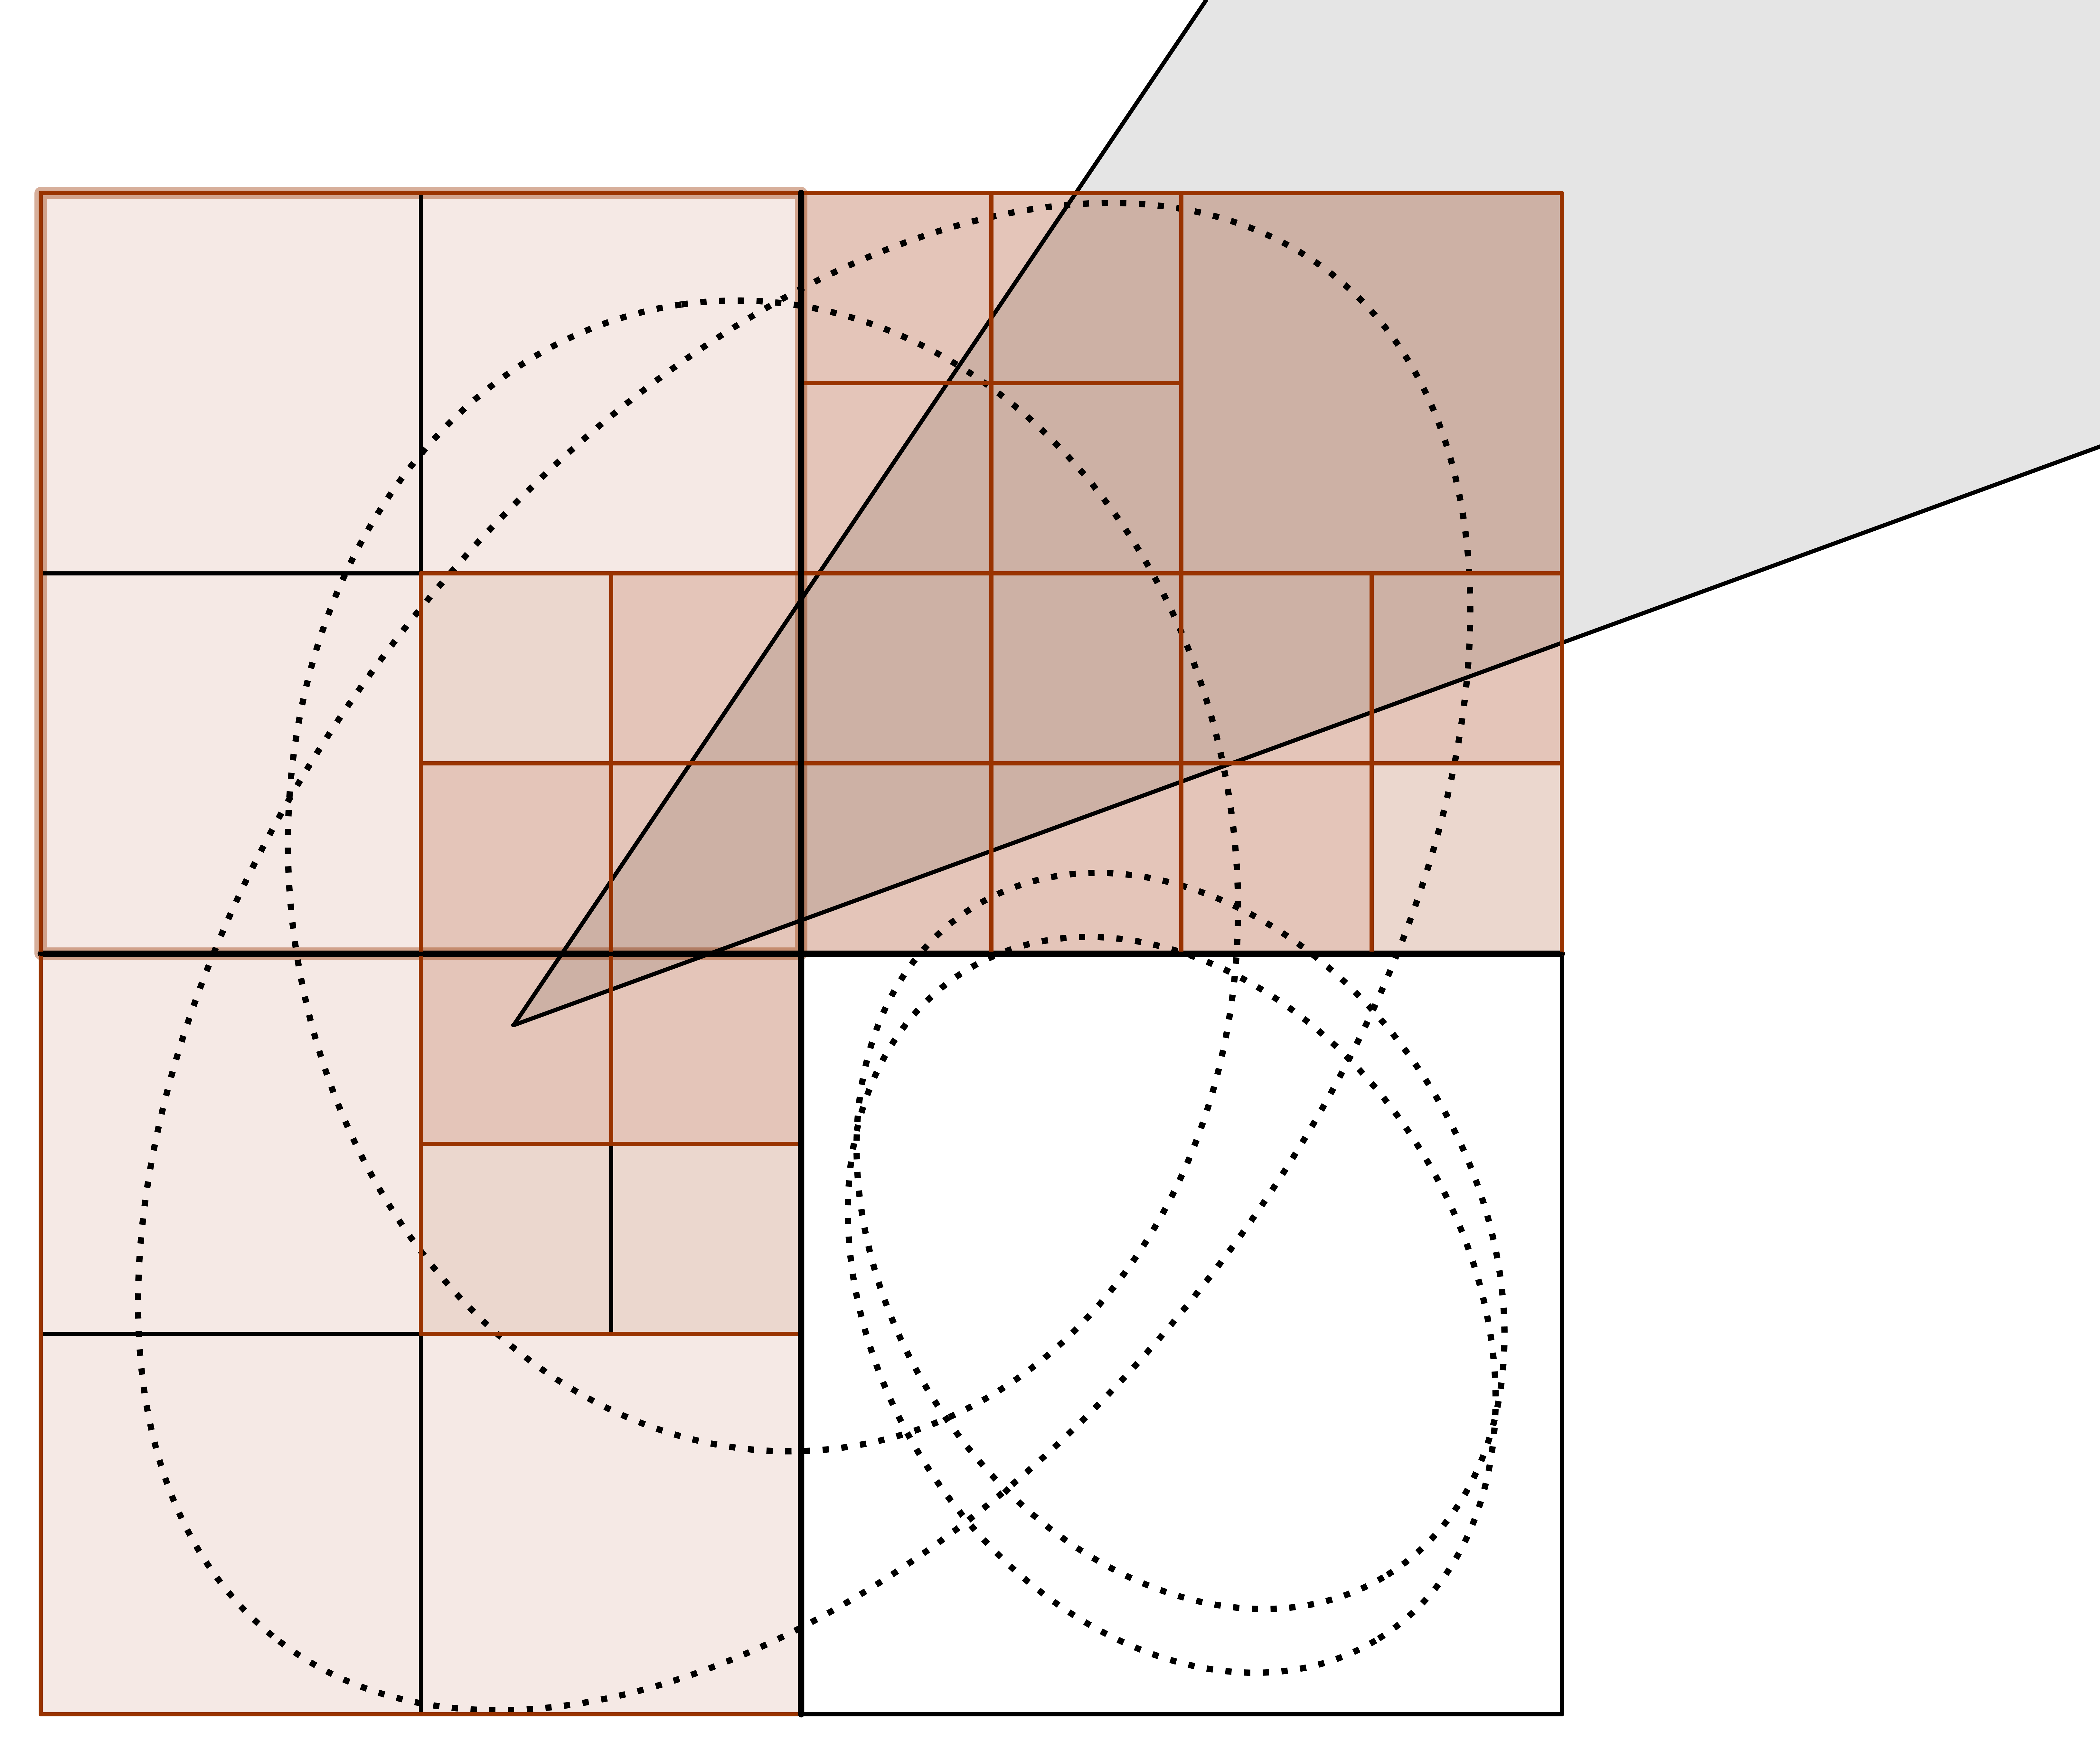
\includegraphics[width=6cm]{octree.png}
\label{fig:octree}
\end{wrapfigure}
The recursive algorithm starts with the \emph{root cuboid}. If it is completely inside the view frustum, the full set of points for that cuboid is extracted. If it is partially inside the view frustum and not a leaf, the algorithm recursively descends into the child cuboids. It it is completely outside the view frustum, the cuboid is discarded. So unlike for the \emph{cubes structure}, large parts of the model can be immediately either included or excluded. The sizes of the cuboids change exponentially with the depth in the tree, so it is very well possible to immediately exclude over half of the model, but be very precise inside the frustum.

\subsubsection{Extra splits}
Including a cuboid means that the set of points inside that cuboid is copied to the output buffer. As described before, these points are always on a single data segment. The downsampling level $\ell$ for this cuboid is chosen using a \emph{point-to-cuboid} distance, as described before. However there is the problem that if large cuboids are to be included, choosing a single downsampling level for it will not be appropriate.

Therefore, the algorithm further recursively splits such cuboids, as long as the difference between its \emph{maximal} and \emph{minimal} \emph{point-to-cuboid} distances is larger than a given threshold. This difference corresponds to the two extrema where $r(d)$ would be most different.

\subsubsection{Load order}
The algorithm described here does not specify in which order the children of a cuboid should be traversed. This becomes a problem when the \emph{downsampling setting} is not sufficient, and the algorithm stops at some instant during the recursions because the capacity $C$ has already been filled. Then it can happen that parts of the model farther to the camera are rendered, but closer parts are lost.

If such an overflow occurs, it is preferential to first render the closer parts, and maybe drop the points in the background.\footnote{This is especially true when occlusion culling is added.} A modified, ``ordered nodes'' version of the algorithm does this.

Firstly, when traversing the child cuboids of a cuboids, the algorithm first sorts them by their \emph{point-to-cuboid} distances to the camera, and recurses into the closer ones first.

In addition to this, it must no longer begin with the \emph{root cuboid}, but rather begin at the \emph{leaf} containing the camera, and then move outward. This is mostly an optimization, but in some cases, for instance when the \emph{minimal} \emph{point-to-cuboid} distance is chosen, it is necessary to prevent the algorithm from moving down the wrong node.

Also as a small optimization, the algorithm stores the current node containing the camera and tracks as the camera moves into parent or neighboring nodes.

\subsection{Creation algorithm}
The following describes the procedure taken to create a tree structure. First the bounds of the model are determined by finding the minima and maxima of the points' coordinates. An enclosing cuboid (adjusted to \emph{include} all points, and to fit needs of splitter) is created.

Recursively, starting with the root node, these steps are taken: The list of points from the current node $p \in \mathcal{C}$ is used to calculate the \emph{node points information}. Then, the points are distributed into $c$\footnote{number of children per node} new lists according which child node they belong. At this point, the algorithm requires memory for two times the full list of points. This is necessary because the algorithm that calculates \emph{node points information} for the \emph{KdTree-Median} requires a list of points. It also simplifies things because the numbers of points are always known, and with it whether a node will be a leaf.

The full points list is now no longer needed and memory can be released. Using the \emph{node points information}, cuboids for the child nodes are computed. Then the child node points lists are used to recursively execute the same process in each child node. The recursion stops when the number of points is smaller than the \emph{leaf capacity}, and the \emph{leafs} store their points in an internal buffer. So at the end, each point exists exactly once in memory, in a leaf's buffer.

The points used as input for the whole algorithm don't come in any specific order. Their required final order (for extraction of node points as segment) can be known only after the full tree, i.e. the numbers of points in each node, is determined. So the second phase is to \emph{move out} the points from the leaves' buffers into a global list of points.

A depth-first descent into the tree is done, and for each leaf its points are appended to the global list. During traversal, each node stores the current length of the global list: It will become the offset in the list of the segment that contains the points of that node. The recursive descent is also used to sum up the numbers of points for non-leaf nodes.

\subsubsection{Downsampled points}
Adding downsampled points to the tree structure is easier because the nodes of the tree and their cuboids have already been determined.

Unlike with the \emph{cubes structure}, the downsampling algorithm is applied to the entire set of points. The leaves likely have not enough points to allow for good quality downsampling. Then each point in the resulting set $P'$ is added into an internal buffer (for that downsampling level) of a leaf.

Even though the downsampled point set always contains fewer points than the full points set, it is possible that within a given cuboid there will be more points: Uniform downsampling will produce different points than there were in the input, so this is unpredictable on a local level. As a consequence it occurs sometimes that points don't fit into the capacity of the leaf's internal buffer.

In that case the buffer is increased. The algorithm must not delete points because the total number of downsampled points in the structure must be predictable. (explained later)

After this the points are \emph{moved out} the same way as for the original point set, so as to create the ordered list.


\section{Piecewise tree structure}
The entire algorithm described before aims at creating the tree structure \emph{in memory}, and so the maximal model size is limited. Also, it requires much more memory during the process than the final structure will take (internal/temporary buffers, etc.)

Exporting the \emph{in-memory} tree structure into an HDF file is relatively straightforward. In order to allow for huge models to be ``streamed'' from the raw point set to an HDF file containing the tree structure, the idea used is to construct several temporary tree structures in memory that contain only a \emph{piece} of the model, and to combine them into a complete tree structure in the HDF file.

Since the goal is to end up with a large \emph{tree} structure, the pieces will be cuboids of leaves on a outer ``meta-tree'' created from the full point set. In this text, the term \emph{outer tree} denotes that tree, whereas the term \emph{inner tree} denotes the temporary tree structure built for a \emph{piece}.

As described in \ref{sec:tree_ser}, the structure of the \emph{HDF} representation allows the \emph{outer} and \emph{inner} trees to be created by different rules. This is useful because the \emph{inner} trees will subdivide the model into very small regions and aim for high visual output quality, making the \emph{Octree} a good choice.

In contrary, the \emph{outer} tree will have very large leaves, and the number of points in the leaves should be controllable: It should be as small enough so that the \emph{inner} tree structures will still fit in memory, but there should not be too many small pieces. The \emph{KdTree-Half} is a good choice here because it subdivides by two instead of by eight, so there is no explosion in the number of pieces.

The \emph{KdTree-Median} might be a better choice since it equalizes the number of points in its children, but is not usable here because the entire points set can't be loaded into memory to calculate a median.

\subsection{Building the outer tree}
The outer tree will not store any points in memory, but just the nodes and cuboids information. It cannot be built the same way as described before (normal tree structure, aka \emph{inner} trees), because there temporary lists of points are kept. An analogue algorithm that does not keep lists in memory would need to read through the entire input file (containing the full point set) at each recursion, and consider only the points in its cuboid. This would be very inefficient. Also an algorithm in which leaves are turned into nodes as new points get added is not possible because no information is kept about the points in the leaves.

Instead, the algorithm begins by building a tree where every node has $c$ children, down to a predefined depth $d_{\max}$. All nodes have an internal counter initialized at zero. Then the program reads through the file, and for each point, increments the counters in \emph{all} of the nodes down to the leaf in which the point belongs. In case the counter of a leaf gets greater than $k$\footnote{The leaf capacity of the outer tree, aka the maximal number of points there can be in a \emph{piece}.}, the entire algorithm must restart, this time with a larger maximal depth $d_{\max}$.

After this has succeeded, the program traverses the nodes, and if a non-leaf node has less than or exactly $k$ points, it removes its children and turns it into a leaf. The resulting tree now represents the outer tree. The sum of the numbers of points in the leaves necessarily corresponds to the total number of input points and so the (theoretical) data offsets for an ordered points list can be calculated. The leaves of this outer tree will be the \emph{pieces} of the piecewise tree structure.

\subsection{Building the inner trees}
For each \emph{piece}, an inner tree is built the same way as described for the ``normal'' tree structure; except that only the points that lie inside the cuboid of the piece are taken from $P$.

\subsection{Combining the trees}
After the outer tree is built, the program starts by writing its nodes information into the HDF file, by recursively traversing it. When a leaf is reached, it builds the temporary inner tree, and then writes its nodes and points into the file.

The offsets by which a node in the inner tree refers to its child nodes in the \texttt{nodes} \emph{HDF} data set must be ajusted by adding the offset in the global nodes list where the inner tree's nodes list is appended.

For the points data offsets associated to outer tree nodes, the algorithm just needs to keep track of the current length in the points list. The point sets from the different inner trees are concatenated one after the other.


\section{Parallelized piecewise tree creation}
Because the inner trees are independent from each other (except the absolute offsets after adjustment), the same mechanism can be also be used to parallelize the creation of a tree structure, by constructing several inner trees simultaneously. This again increases memory usage, but can cut the execution time by more than half.

The main problem is that both the number of nodes and the number of points in the inner trees are only known after the tree is built, but these lists need to be concatenated right after each other in the final \emph{HDF} file.

The nodes may be listed in the \emph{HDF} file in any order, as explained in \ref{sec:tree_ser}. So the tasks that create inner trees will just store the inner tree's nodes list separately in memory. After all inner trees have been created, their nodes lists are adjusted (offsets, etc.) and concatenated into the final list, in a sequential postprocessing stage.

However, the points data needs to be in the correct order. There also cannot be gaps in the data because then the points corresponding to outer tree nodes would no longer be in a contiguous segment. The reason why the length of the inner tree's point sets is not known in advance is because both they depend on the output of the random and uniform downsampling algorithms (see \ref{sec:downsampling}).

Because of this random downsampling is implemented in a manner so that the exact number of points to output can be specified. For uniform downsampling, the program resorts to making the uniform downsampling algorithm yield a slightly smaller-than-requested output quantity, and then fills the set up with duplicates of randomly chosen points from itself.

With the number of downsampled points that the inner tree structures will contain being now known in advance, it is possible to in advance allocate the right segment in the complete \emph{HDF} points set for the results to be produced by the different inner structures.


\chapter{Implementation}
The implementation consists of two parts:
\begin{description}
\item[Library] The \emph{Dynamic Point Cloud Library} (\texttt{dypc}) implements all of the data structures and algorithms described here. It provides an API interface to load models from \emph{PLY}\footnote{File format used to store output from 3D scanners} files or generate example models, to create data structures containing a model, store it in a file, and to dynamically load points out a data structure stored in memory or in a file.
\item[Viewer] An application that renders the point cloud and provides a graphical user interface for traveling through the point cloud, and to create and load different data structures. It uses the \texttt{dypc}.
\end{description}

\section{Library}
The shared library is implemented in \emph{C++}, using the \emph{STL} standard template library, and \emph{GLM} for mathematical helper functions. It also uses the C/C++ libraries for \emph{HDF5} and \emph{SQLite}. Because of its use of template metaprogramming, a lot of symbols are generated when compiling. All of the \emph{C++} symbols have \emph{hidden} visibility and are for internal use inside the library only. It provides a small pure \emph{C} interface for the API. This avoids problems with linking different \emph{C++} binaries, minimizes coupling, and allows for the library to be used from other programming languages. It is implemented in a mix of object-oriented, procedural and generic programming similar to the \emph{STL}.

\subsection{Overview}
The following main classes or components compose the library:
\begin{description}
\item[model] A model is a source of input for points. There are subclasses for reading points from a \emph{PLY} file, or for generating random example models. Points can be read from it via an iterator interface. Additionally, it is possible to read from two different iterators simultaneously, for multi-threading use. For the \emph{PLY} file \emph{model}, this is implemented using multiple file handles. The \emph{model} itself does not store any points in memory (apart from internal buffers).
\item[ply\_model] Reads from a \emph{PLY} file. Limited support for \emph{PLY} (e.g. no ASCII files), optimized for speed.
\item[random\_model] Abstract base class for model generated based on random number generator. The \emph{seed} of the random number generator acts as ``file handle''. Used for the example models \textbf{concentric\_spheres\_model} and \textbf{torus\_model}.
\item[structure] Abstract base class for a data structure. Objects of this class contain the data structure in memory and provide an interface for \emph{loaders} to access it. Remains linked by reference to its \emph{model}. The subclass constructors implement the creation of the data structure from the model.
\item[mipmap\_structure] Abstract base class for a data structure that uses \emph{LOD regions}, aka \emph{mipmaps}. Provides access to downsampling algorithms and functions to determine downsampling ratios/levels.
\item[loader] Abstract base class for a \textbf{loader}. See below.
\item[cubes\_structure] Cubes stucture, \emph{weighted points} variant.
\item[cubes\_structure\_loader] Abstract base class for \emph{weighted points} cubes structure loader. Subclasses for \emph{HDF}, \emph{memory}, \emph{SQLite} exist.
\item[cubes\_mipmap\_structure] Cubes stucture, \emph{LOD regions} variant.
\item[cubes\_mipmap\_structure\_loader] Abstract base class for \emph{LOD regions} cubes structure loader. Subclasses for \emph{HDF} and \emph{memory} exist.
\item[tree\_structure, etc] Classes for tree structures, see below.
\item[downsampling] The downsampling algorithms, and level/ratio functions.
\end{description}

\subsection{Loader}
A loader exists for each data structure, and possibly both for reading from a file and from memory (aka from the \emph{structure} object). It implements the \emph{extraction algorithm}, which generates the filtered point set $P'$ from its source. The \emph{request} to the loader consists the current camera position, orientation, view frustum. Movement velocity is also included but not used by and loader. In addition, the capacity $C$, and loader-specific parameters such as the \emph{downsampling setting} $s$, and the \emph{point-to-cuboid} distance mode are also given as input.

It writes the outputted points into a provided buffer. In the \emph{Viewer}, this is virtual memory mapped directly to an OpenGL GPU buffer.

The \emph{direct\_model\_loader} extracts points directly from a \textbf{model} without any filtering or data structure.


\subsection{Tree structure}
Tree structures are implemented by the \textbf{tree\_structure} template class.\footnote{Many other classes used are template classes as well.} It is parametrized by a \emph{splitter} class, which is a subclass of \textbf{tree\_structure\_splitter} with only static members. The \emph{splitter}'s \texttt{number\_of\_node\_children} const static member determines how many children nodes shall have. This is implemented using meta-programming to avoid additional heap allocations required for a runtime-determined number of children.

Its \emph{point container} can either be the \emph{STL} \texttt{vector} or \texttt{deque}. Reading and writing to \texttt{vector} is faster, but it needs to allocate large contiguous memory segments which may fail. \texttt{deque} uses an internal chunked structure.

The tree structure node template class \textbf{tree\_structure\_node} works in conjunction with \textbf{tree\_structure}. It also provides access functions to loaders. \textbf{tree\_structure} can load (and generate) and unload points for the different downsampling levels, and create the structure only for a given cuboid.

This is used for its subclass \textbf{tree\_structure\_piecewise}, which essentially implements outer tree creation on piecewise tree structures. The underlying \textbf{tree\_structure} will be made to contain one inner tree structure. \textbf{tree\_structure\_piecewise} can also spawn a new \textbf{tree\_structure} that contains one piece. This is used for the parallelized implementation.

There are two loader variants: \textbf{tree\_structure\_simple\_loader} and \textbf{tree\_structure\_ordered\_loader}. The latter implements the improved extraction algorithm by which the cuboids closer to the camera are loaded first.

The \emph{tree loader sources} \textbf{tree\_structure\_memory\_source} and \textbf{tree\_structure\_hdf\_source} provide a polymorphic interface for loading from either an in-memory structure or an \emph{HDF} file.

Exporting the tree structure to \emph{HDF} is implemented in \textbf{tree\_structure\_piecewise\_hdf\_write} and the parallelized version \textbf{tree\_structure\_piecewise\_hdf\_write\_parallel}. The \textbf{tree\_structure\_hdf\_file} class provides the basic structure for reading and writing to \emph{HDF}. There is an optimization for copying segments of points directly out of a \texttt{vector}.


\subsection{Additional parts}
\begin{description}
\item[structure\_loader\_factory] Functions for creating loaders, writing to files, etc. Essentially map parameters to template parameters.
\item[interface] The \emph{C} API interface to the library. Only these functions are exported.
\item[geometry] Implementation of geometry algorithms and objects such as cuboid, frustum, plane.
\item[sqlite] An \emph{SQLite} wrapper.
\item[point, weighted\_point] POD class types for POD \emph{points}. Meant to be copied directly across \emph{HDF}, memory and \emph{GPU} video memory.
\item[progress] Helper functions for displaying progress bars. Interface provides callbacks for GUI.
\item[utils, debug, enums] Some helper functions.
\end{description}


\pagebreak

\section{Viewer}
The \emph{Viewer} is also implemented in \emph{C++}. It uses the \emph{wxWidgets} toolkit to provide a graphical user interface. The main reason for choosing \emph{wxWidgets} was to have a \emph{C++} based, cross-platform GUI with support for including \emph{OpenGL} render context in a window.
\emph{OpenGL} is used for the rendering, and the \emph{GLM} library is also used. The \emph{Viewer} links with the \emph{dypc library} and provides a graphical user interface to all of its functionality. The forms are created using \emph{wxFormBuilder}, which generates \texttt{.cpp / .hpp} files the form automatically.

\subsection{Streaming mechanism}
The \emph{Viewer} attempts to provide the user with a seamless experience in that they can move through the virtual point cloud, while the program dynamically loads visible point sets $P'$. The application uses two threads: The main thread operated the user interface and OpenGL renderer, while the secondary thread runs the \emph{updater} which periodically sends new requests to the \emph{loader} in the \emph{dypc library}, and passes the new point sets to the renderer.

To make this last step efficient, a \emph{buffer swap} mechanism is used: Two OpenGL point buffers are allocated in video memory with the same point capacity $C$. The \emph{renderer buffer} is used by OpenGL for the rendering, while the \emph{loader buffer} is being filled by the loader. The use of virtual memory mapping and the \emph{POD} \textbf{point} type makes it possible to directly copy raw data from the loader to the GPU. The \textbf{point} is composed in such a way that \emph{OpenGL} can directly extract the coordinate and color data from the raw data. In some cases, it is possible that point data is stored in the \emph{HDF} files in exactly the same binary format, and can also be copied directly to the buffer.

The \emph{buffer swap} occurs when the updater has finished filling the \emph{loader buffer}. It then notifies the render that new data is available via an atomic flag, and waites for a new request. Once available, the \emph{renderer} swaps the two buffers: The \emph{loader buffer} becomes the new \emph{renderer buffer} and vice versa. So no copy takes place, and there is no interference between \emph{renderer} and \emph{updater}. Several concurrency facilities such as mutexes and atomic types are used in the implementation.

\subsection{Renderer}
The \emph{renderer} is responsible both for making \emph{OpenGL} render the data in the \emph{point buffers}, and for allowing the user to move through the virtual space.

It is implemented in \emph{OpenGL 4}, so \texttt{glDrawArrays} is used to render data and the projection math is implemented using \emph{GLSL} vertex and fragment shaders. There also implement a visual \emph{fog} effect, and the \emph{point shadow} occlusion culling.

\section{Usage}
Movement through the point cloud is controller with the \texttt{Z, Q, S, D} keys. \texttt{Space} moves up, and \texttt{<} moves down. The speed can be set on the right panel. The camera orientation can be changed by holding and dragging the mouse in the renderer area. The scroll wheel rolls the camera.

\subsection{Compilation}
Both the \emph{library} and \emph{viewer} are built by issuing \texttt{make} in the \texttt{app} directory. The viewer, along with \texttt{libdypc.so} will be located in \texttt{dist/viewer}. Setting \texttt{DEPLOY = 1} in the Makefile disables assertions and enabled compiler optimizations. It makes the program much faster.

The following external dependencies (libraries and development headers) are required:
\begin{itemize}
\item GCC compiler with full C++11 support
\item OpenGL and GLEW
\item wxWidgets, at least version 2.8.
\item SQLite3
\item HDF5 CPP
\item GLM
\item The wxFormBuilder program
\end{itemize}

The \emph{Viewer} displays its progress indicators in the console. A GUI version exists, but is not activated because proper support for multi-threading is not implemented for the parallelized tree creation is not implemented. Also the \emph{Viewer} does not verify all user input, and does not handle all error conditions reported by \emph{dypc}.


\subsection{Example files}
The \texttt{ply} directory contains some \emph{PLY} models. \texttt{tower.ply} is a huge colored point cloud containing about 150 million points. Smaller downsampled versions are also included.

The \texttt{hdf} directory contains some different \emph{HDF} files with structures created from these models. They can be visualized in the \emph{viewer}.


\appendix
\chapter{Geometric algorithms}

\section{Definitions}
The geometric objects used in the algorithms are defined in the following manner:
\begin{description}
\item[cuboid] Axis-aligned cuboid $\mathcal{C}$ is defined by \emph{origin} point $x, y, z$, and \emph{extremity} point $x', y', z'$, such that $x' > x$, $y' > y$ and $z' > z$. The coordinate intervals are open on the extremity side, i.e. a point $\overrightarrow{p}$ is considered to be inside the cuboid if and only if $p_{x} \in [x, x'[$, $p_{y} \in [y, y'[$ and $p_{z} \in [z, z'[$. See section \ref{sec:cub_reg} for further explanation.

\item[plane] An oriented two-dimensional plane $P$ in three-dimensional space is defined using four real values $a, b, c, d$. $\overrightarrow{n} = (a, b, c)$ is a normal vector of the plane, while $d$ is the distance from the origin to the plane, multiplied by $|\overrightarrow{n}|$.

In its \emph{normalized} form, $a, b, c, d$ are defined such that $|\overrightarrow{n}| = 1$. Then $d$ is simply the distance from the origin to the plane, and each plane there is exactly one normalized form.

The planes are oriented, that is an (oriented) distance from a point $\overrightarrow{p}$ to the plane is positive when $\overrightarrow{n} \cdot \overrightarrow{p} \geq 0$, and negative otherwise. If it is positive, the points is called \emph{in front of} the plane, and otherwise it is \emph{behind} the plane.

\item[frustum] A frustum is defined using the 6 planes that delimit it: the near, far, left, right, top and bottom planes. Supposing that the normal vectors of the planes are all pointing inside the frustum, a point is considered to be inside the frustum if and only if its oriented distance to each one of the planes of positive.

This representation of a frustum not unique, and is only valid when the 6 planes are arranged so as to delimit a frustum. A frustum can be defined using a 4x4 projection matrix, and the following algorithm describes how to get the 6 planes out of it.
\end{description}

\section{Projection matrix to view frustum} \label{frustum_planes}
Let $\matrixsym{M}$ be a projection matrix, and $\matrixsym{M}[i, j]$ be the value in $\matrixsym{M}$ at column $i$ and row $j$, counting from 0.
As described in \cite{Gri2001}, the 6 planes $P = (a, b, c, d)$ can be derived as follows:
\begin{align*}
	P_{\text{near}}   = (\matrixsym{M}[0, 3] + \matrixsym{M}[0, 2], \quad \matrixsym{M}[1, 3] + \matrixsym{M}[1, 2], \quad \matrixsym{M}[2, 3] + \matrixsym{M}[2, 2], \quad \matrixsym{M}[3, 3] + \matrixsym{M}[3, 2]) \\
	P_{\text{far}}    = (\matrixsym{M}[0, 3] - \matrixsym{M}[0, 2], \quad \matrixsym{M}[1, 3] - \matrixsym{M}[1, 2], \quad \matrixsym{M}[2, 3] - \matrixsym{M}[2, 2], \quad \matrixsym{M}[3, 3] - \matrixsym{M}[3, 2]) \\
	P_{\text{left}}   = (\matrixsym{M}[0, 3] + \matrixsym{M}[0, 0], \quad \matrixsym{M}[1, 3] + \matrixsym{M}[1, 0], \quad \matrixsym{M}[2, 3] + \matrixsym{M}[2, 0], \quad \matrixsym{M}[3, 3] + \matrixsym{M}[3, 0]) \\
	P_{\text{right}}  = (\matrixsym{M}[0, 3] - \matrixsym{M}[0, 0], \quad \matrixsym{M}[1, 3] - \matrixsym{M}[1, 0], \quad \matrixsym{M}[2, 3] - \matrixsym{M}[2, 0], \quad \matrixsym{M}[3, 3] - \matrixsym{M}[3, 0]) \\
	P_{\text{bottom}} = (\matrixsym{M}[0, 1] + \matrixsym{M}[0, 1], \quad \matrixsym{M}[1, 3] + \matrixsym{M}[1, 1], \quad \matrixsym{M}[2, 3] + \matrixsym{M}[2, 1], \quad \matrixsym{M}[3, 3] + \matrixsym{M}[3, 1]) \\
	P_{\text{top}}    = (\matrixsym{M}[0, 1] - \matrixsym{M}[0, 1], \quad \matrixsym{M}[1, 3] - \matrixsym{M}[1, 1], \quad \matrixsym{M}[2, 3] - \matrixsym{M}[2, 1], \quad \matrixsym{M}[3, 3] - \matrixsym{M}[3, 1])
\end{align*}

\section{Maximal point-to-cuboid distance}
The maximal distance from a point $\overrightarrow{p}$ to a cuboid $\mathcal{C}$ is always the distance to one of the 8 corners of $\mathcal{C}$ (also if $\overrightarrow{p}$ is inside $\mathcal{C}$). The algorithm simply tests the distances from $\overrightarrow{p}$ to each one of the corners and returns the maximal one. As a small optimization, the algorithm can compare the squares of the distances instead, so as to do only one square root computation.

\section{Minimal point-to-cuboid distance}
The minimal distane from a point to a $\overrightarrow{p}$ to a cuboid $\mathcal{C}$ can either be the distance to one of the corners of $\mathcal{C}$, or the distance to one of its edges, or one of its sides. If $\overrightarrow{p}$ is inside $\mathcal{C}$, the distance is always $0$. However there is no need to explicitly distinguish all those cases:

Let $\overrightarrow{d} = (\Delta x, \Delta y, \Delta z)$ be the vector from $\overrightarrow{p}$ (point) to the point on $\mathcal{C}$ such that $d = |\overrightarrow{d}|$ is minimal. If $p_{x} \in [x, x']$, then $\overrightarrow{d}$ will point straight to $\mathcal{C}$ in the $x$-direction, so $\Delta x = 0$. If $p_{x} < x$, it needs to turn towards $\mathcal{C}$, so $\Delta x = p_{x} - x$. Same for when $p_{x} > x'$, then $\Delta x = -(x' - p_{x})$.

The coordinates $\Delta y$ and $\Delta z$ are determined the same way. Finally $d = \sqrt{\Delta x^{2} + \Delta y^{2} + \Delta z^{2}}$ is calculated. This implies that $d$ will be set to $0$ when $\overrightarrow{p}$ is inside $\mathcal{C}$. A small optimization might be to avoid calculating the square and square root when none or only one coordinate is non-zero.

\section{Frustum-cuboid intersection}
To test whether a cuboid is inside or outside the frustum, is is not sufficient to test if any corner of the cuboid is inside the frustum, because if the cuboid completely encloses the frustum, all of its corners will be outside, but the cuboid still intersects the frustum.

Considering that the 6 planes of the frustum are oriented towards the inside of it, a cuboid is inside the frustum, if for every one of the 6 planes, at least one corner of the cuboid is in front of it. This is obviously true when at least one point of the cuboid is inside the frustum, but also when any position inside the cuboid is inside the frustum. Also, if all 8 corners are behind any one plane, then the cuboid must be outside the frustum.

So the algorithm that distinguishes inside and outside is as follows:

\begin{algorithmic}
	\ForAll{plane $P_{i}$}
		\ForAll{corner point $c_{j}$}
			\If{$c_{j}$ is in front of $P_{i}$} \textbf{continue} \\
				\Comment{$c_{j}$ is in front of $P_{i}$. No need to check other corners.} 
			\EndIf
		\EndFor \\
		\Return false \Comment{All corners were behind $P_{i}$, so $\mathcal{C}$ is outside}
	\EndFor \\
	\Return true \Comment{All planes had a corner in front of them, so $\mathcal{C}$ is inside}
\end{algorithmic}

Because the frustum is not a cuboid (the planes are not all parallel, so somewhere they intersect and change orientation), this algorithm can sometimes produce false positives. If is possible for all planes to have a corner in front of them yet the cuboid is not inside the frustum. But this only rarely occurs in an area behind the frustum, and does not pose a practical problem.


\section{Frustum-cuboid (partial) intersection} \label{sec:fr_cub_inter}
The algorithm can be extended to distinguish 3 cases: If the cuboid is completely outside, partially inside, or completely inside the frustum. A cuboid is completely inside the frustum only if all its corners lie inside the frustum. The following is an extended version of the previous algorithm that also checks, for each plane, whether \emph{all} corners lie in front of it.

\begin{algorithmic}
	\State $p \gets 0$ 
	\Comment{$p$ counts planes that have all 8 corners in front}
	\ForAll{plane $P_{i}$}
		\State $c \gets 0$
		\Comment{$c$ counts corners in front of $P_{i}$}
		\ForAll{corner point $c_{j}$}
			\If{$c_{j}$ is in front of $P_{i}$}
				\State $c \gets c + 1$
			\EndIf
		\EndFor
		\If{$c = 0$}
			\Return{completely outside}
		\ElsIf{$c = 8$}
			\State $p \gets p + 1$
		\EndIf
	\EndFor
	\If{$p = 6$}
		\Return{completely inside}
	\Else
		\Return{partially inside}
	\EndIf
\end{algorithmic}


\bibliographystyle{plain}
\bibliography{report}


\end{document}
